%!TEX root = ../../../adrien_gomar_phd.tex


\subsection{Highlighting the problem}

\paragraph{Rectangular function}

In fluid dynamics, the simplest model 
representative of a shock wave
is the step function.
In fact, in a
shock, the variables present a discontinuity
that can be, at first order, represented by a 
step function. In this study, we will consider for periodicity reasons,
the symmetric version of the step function which is the
rectangular function defined as:
\begin{equation}
    u_0(t) = 
    \begin{cases}
        0, & \text{if } 0 \leq t < \frac{T}{2} \\
        1, & \text{if } \frac{T}{2} \leq t < T.
    \end{cases}
    \label{eq:inject_step}
\end{equation}
The rectangular function is periodized using Eq.~\eqref{eq:periodic_operator}.
% as explained above, since
% it is not periodic in essence.

\begin{figure}[htbp]
  \centering
  \subfigure[$N=1$ computation]{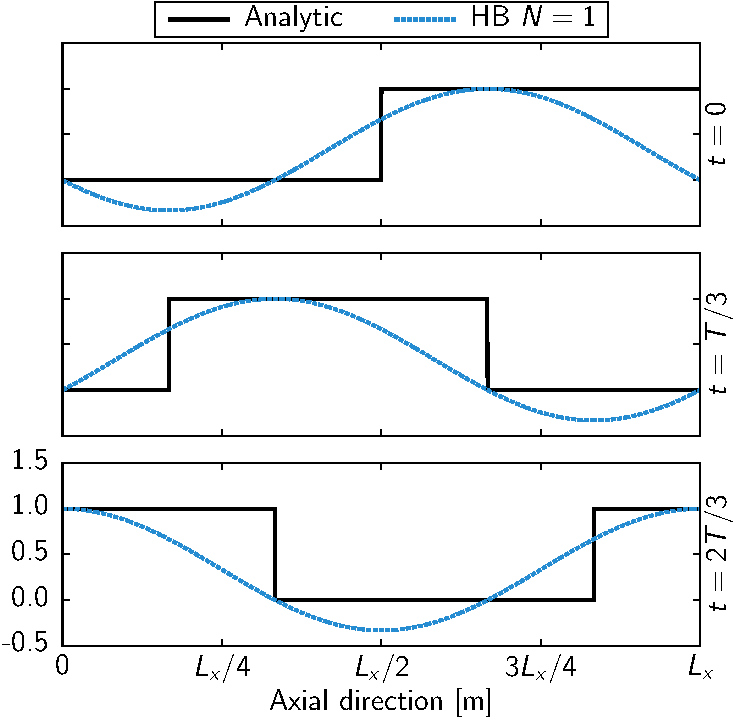
\includegraphics[width=.35\textwidth]{convection_step_N1.pdf}}
  \subfigure[$N=2$ computation]{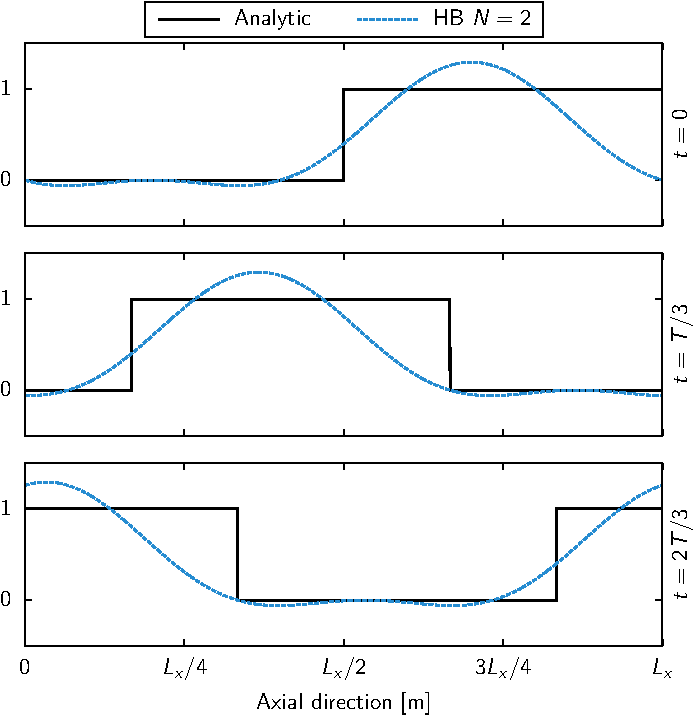
\includegraphics[width=.35\textwidth]{convection_step_N2.pdf}}
  \subfigure[$N=3$ computation]{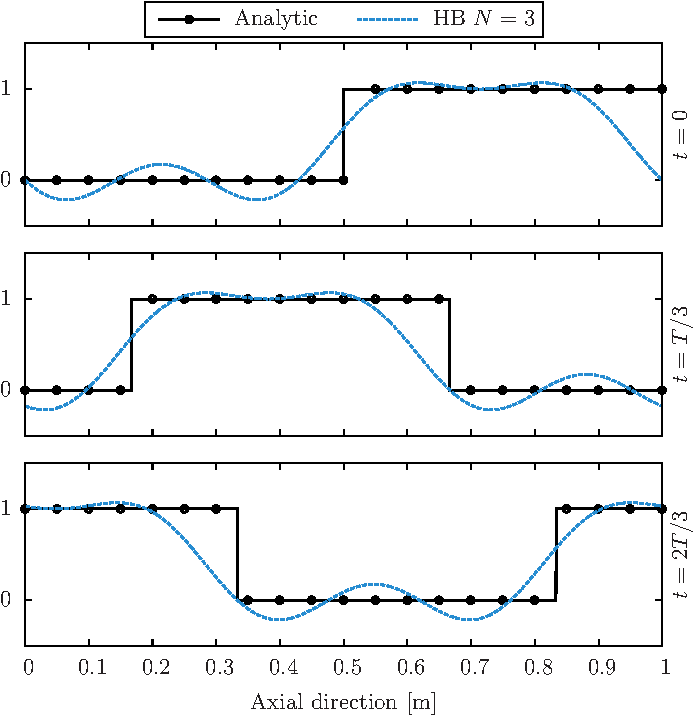
\includegraphics[width=.35\textwidth]{convection_step_N3.pdf}}
  \subfigure[$N=4$ computation]{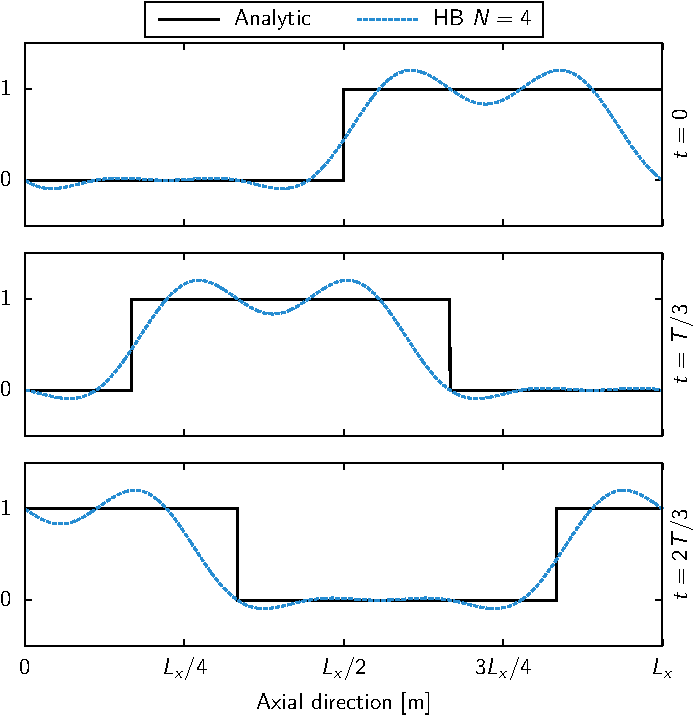
\includegraphics[width=.35\textwidth]{convection_step_N4.pdf}}
  \subfigure[$N=5$ computation]{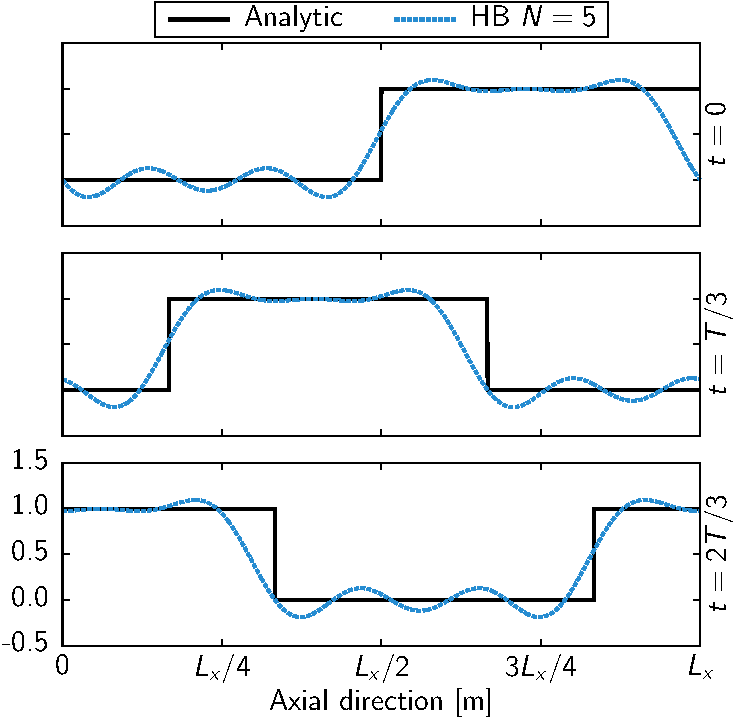
\includegraphics[width=.35\textwidth]{convection_step_N5.pdf}}
  \subfigure[$N=6$ computation]{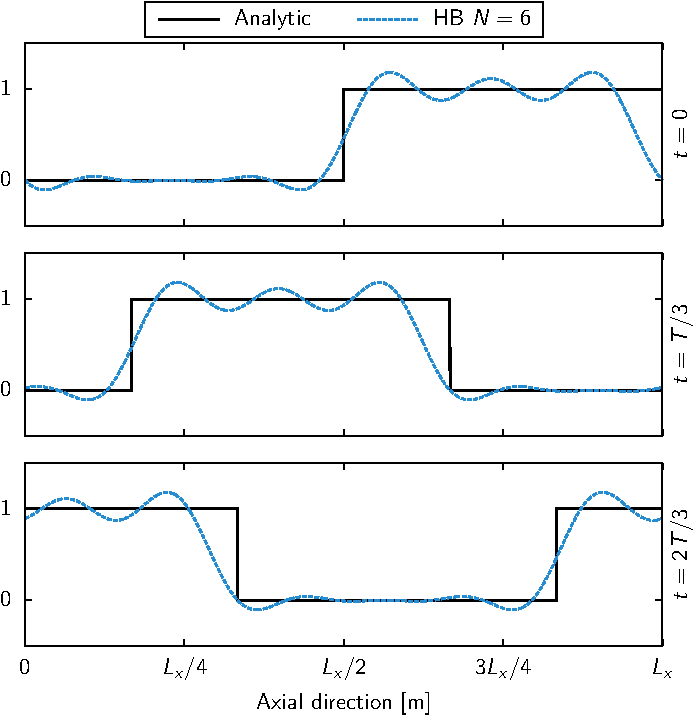
\includegraphics[width=.35\textwidth]{convection_step_N6.pdf}}
  \caption{Harmonic balance results for 
  an injected rectangular function.}
  \label{fig:inj_step_results}
\end{figure}

Figure~\ref{fig:inj_step_results} depicts the harmonic balance
computations from $1$ to $6$ harmonics. The convergence rate 
is slow as for the $N=6$ harmonics computation, the
shape of the rectangular function is still barely captured. 
In fact, the discontinuity is badly captured and a lot of low
oscillations remains. A
\citet{Gibbs1899} phenomenon is also observed which is in agreement with 
the use of Fourier-based methods to capture a discontinuity. This has been
previously observed by \citet{Hembera2009} using
another Fourier-based method, namely the Non-Linear 
Harmonic (NLH) approach~\cite{He1998}.

\begin{figure}[htbp]
  \centering
  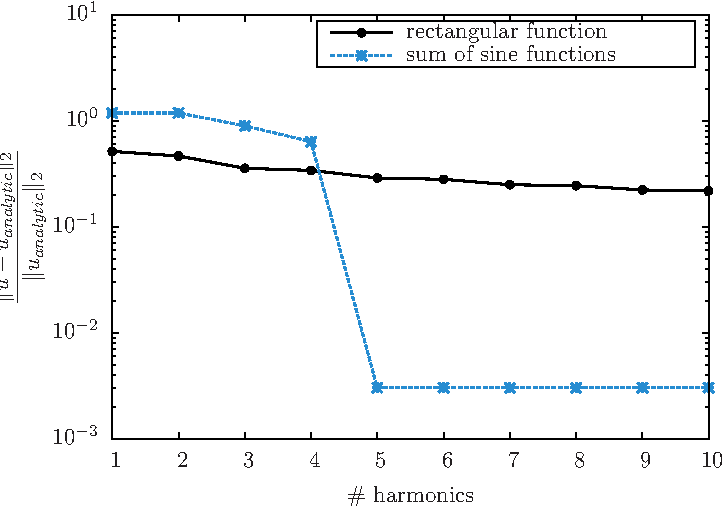
\includegraphics[width=.5\textwidth]{convection_step_error.pdf}
  \caption{Convergence of the harmonic computations for an injected
    rectangular function.}
  \label{fig:conv_step}
\end{figure}
As for the previous sum of sine functions, the $\mathcal{L}_2$-norm 
of the error is depicted in Fig.~\ref{fig:conv_step}. 
The convergence of the sum of sine functions is added for comparison.
The convergence rate is different from the previous one: no threshold phenomenon
is seen, the convergence is monotonic and slow.

To further analyze the convergence, 
the discrete Fourier transform of the results
is computed and depicted against analytical result in Fig.~\ref{fig:dft_step}.
The analytical discrete Fourier transform has
 a cardinal sine shape discrete Fourier transform.
\begin{figure}[htbp]
  \centering
  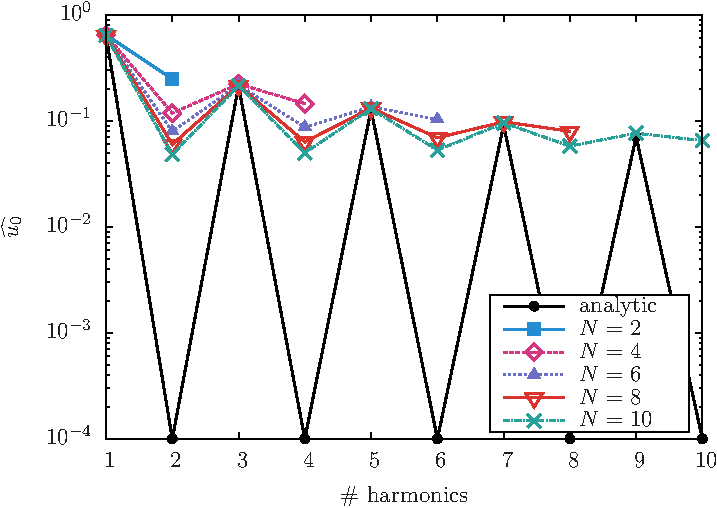
\includegraphics[width=.5\textwidth]{convection_step_dft.pdf}
  \caption{Discrete Fourier transform of the computational
  results compared to the analytical one for an injected 
  rectangular function.}
  \label{fig:dft_step}
\end{figure}
Again, the more harmonics in the computation, the closer the solution
to the analytical results. Surprisingly, only the odd harmonics are
correctly captured while the even ones converge slowly. This might be an
effect due to the shape of the function that is computed. Actually, the odd
sine functions are correctly capturing the shape of the rectangular function, 
as the slope is properly oriented for each stepping part.
\begin{figure}[htbp]
  \centering
  \subfigure[first harmonic]{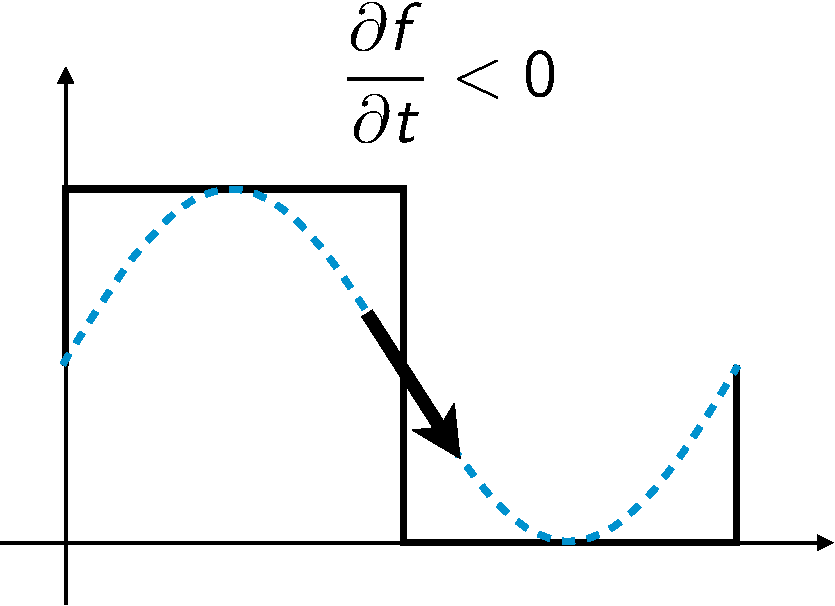
\includegraphics[width=.3\textwidth]{STEP_ODD_EVEN_1.pdf}}
  \subfigure[second harmonic]{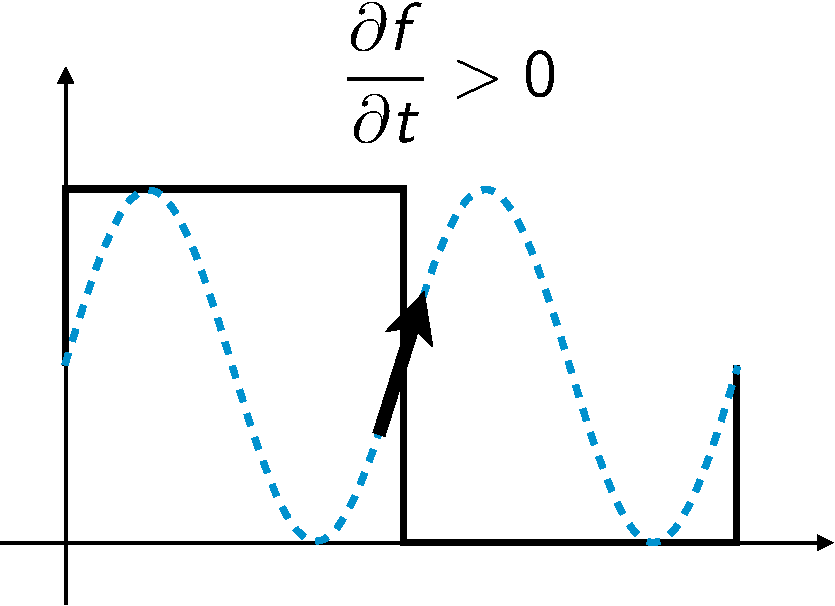
\includegraphics[width=.3\textwidth]{STEP_ODD_EVEN_2.pdf}}
  \subfigure[third harmonic]{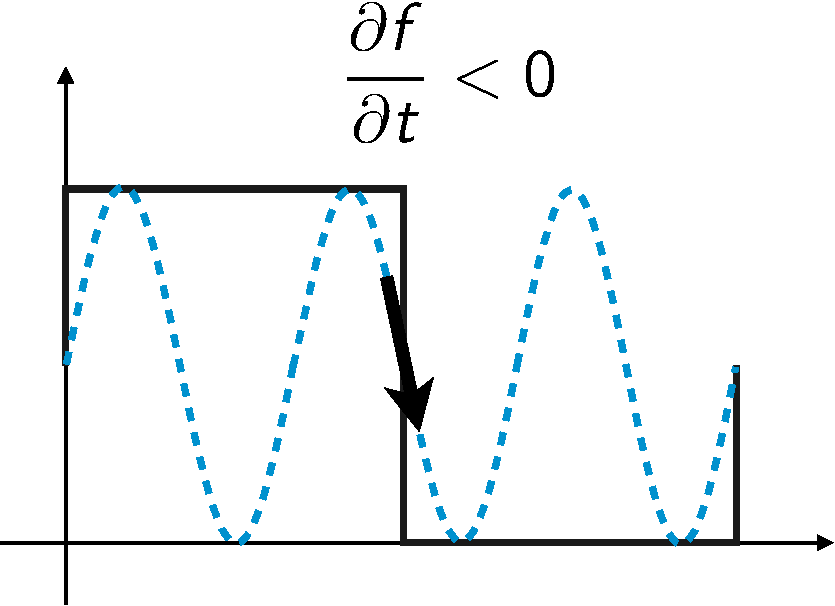
\includegraphics[width=.3\textwidth]{STEP_ODD_EVEN_3.pdf}}
  \caption{Capturing a rectangular function with sine functions.}
  \label{fig:step_conv_sine}
\end{figure}
In Fig.~\ref{fig:step_conv_sine} is depicted the convergence of each harmonic
of a sine decomposition for a rectangular function. 
The derivative of the function is better 
handled by odd sine function than even ones. 
This roughly means that introducing an even sin function
damages the solution.
This explains
why the analytical Fourier transform shows small amplitudes for even harmonics.
However this does not explains why even harmonics converges slowly
in Fig.~\ref{fig:dft_step}. For unresolved computations, as these ones for
instance, the convergence is hard to explain. It looks like some harmonics
retrieve a part of the energy that is not computed since they are
filtered by the Fourier-based method. This behavior was also seen on the
previous case.
Again, the convergence of the computations seems
to follow the shape of the analytical solution as when the number
of harmonics grows, the Fourier transform of the results gets closer
to the analytical Fourier transform.

Let us clarify one important thing here: Fourier-based time integration methods
will show Gibbs phenomenon only if a discontinuity is temporally
present.
This effect can be emphasized by two 
aero-elastic computations that have been performed 
using an harmonic
balance approach. The first one is the case of 
an airfoil with an oscillating 
flap~\cite{JDufour2009}. In this simulation, as the flap is oscillating
under transonic inflow conditions, a shock swings temporally
back and forth from the pressure side to the
suction side. As the discontinuity is
both spatial (a shock is seen on the field) and temporal
(this shock is moving with respect to time), the number
of harmonics needed to capture this phenomenon is
consistent with the capturing of a rectangular function.
Contrarily, two recent publications~\cite{Huang2013, JSicot2012} on the validation
of the use of harmonic balance approach to predict
aero-elasticity damping within turbomachineries, have highlighted
different conclusions. The 11~\textsuperscript{th}
Standard Configuration~\cite{Fransson1999} for aero-elasticity is computed
for validation in both publications. The transonic case
of this configuration shows a passage shock. Under the first bending mode
of the blade, the shock remains steady in the relative frame. As the shock
is only spatial, both publications show a convergence of 
Fourier-based methods with only $N=1$ harmonic. Thus, if the shock
structure is only spatial, Fourier-based methods will not need
extra harmonics to converge, while for a temporally moving discontinuity
(which is the case of our rectangular function), the number
of harmonics to converge will be higher.

Since the present paper focuses on the convergence of turbomachinery
computations, the wake of a blade will be first
simplified and the convergence of harmonic computations will then be
explained.

\paragraph{Towards a turbomachinery wake}
\label{sec:turbomachine_wake}

Consider for generality a stage of a turbomachinery composed of two rotors
with a relative speed difference between the two rows.
Due to the boundary layer that develops on 
the pressure side and the suction side of the blades, a wake is generated behind
the upstream and the downstream rotor. It is stationary in its frame of reference.
\begin{figure}[htb]
    \centering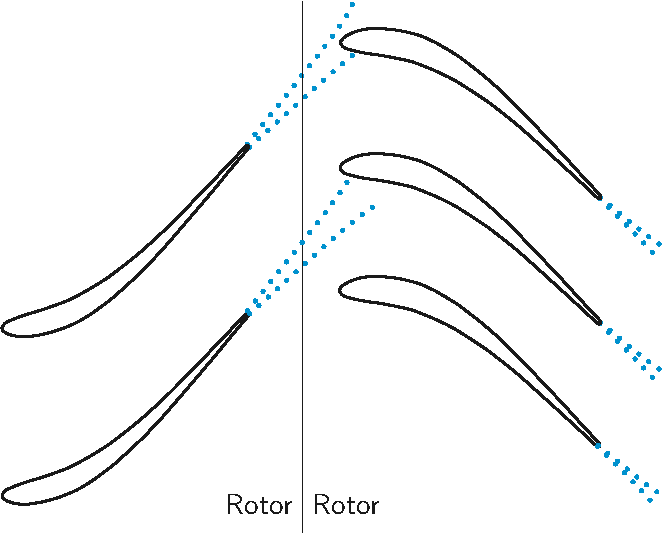
\includegraphics[width=.45\textwidth]{TURBOMACHINES_WAKE.pdf}
  \caption{Characteristic rotor-rotor configuration of a turbomachinery. 
  Wakes are depicted with dashed lines.}
  \label{fig:rotor-stator}
\end{figure}
However, when it crosses the rotor-rotor interface,
the wake becomes unsteady in the downstream rotor frame of reference
because of their relative speed difference. Thus, 
an upstream steady azimuthal heterogeneity becomes unsteady in
the downstream row.

In their pioneer work, 
Lakshminarayana and Davino~\cite{Lakshminarayana1980} showed that the wake
in a turbomachinery follows a similarity law for the velocity. 
It can be statistically estimated by a Gaussian function:
\begin{equation}
    u (\theta) = u_m - 
        \Delta u \cdot e^{
          -0.693 \left( 2 \frac{\theta}{L} \right) ^ 2},
    \label{eq:similarity}
\end{equation}
where $u_m$ denotes the free-stream velocity, $\Delta u$ the axial wake velocity deficit,
$\theta$ the tangential coordinate and $L$ the wake width,
defined as the full width at half maximum.

From the above similarity law and the aforementioned remark on 
the wake becoming unsteady in the downstream row, one can say at 
first order, that the unsteady wake seen by an observer in the downstream row
of reference can be associated with the convection of a periodic 
Gaussian function. The downstream row can be a stator or a rotor,
this holds true for the upstream row. The only condition needed for
this statement to be true, is that a relative motion exists
between the two rows.

The previous convection model problem is now tested
with an injected Gaussian function as defined in Eq.~\eqref{eq:similarity}.
The width $L$ is set to $10\%$ of the domain size $L_x$, 
$u_m$ is set to $1~L_x / c$ and $\Delta u$ to $10\%$ of $u_m$.

\begin{figure}[htbp]
  \centering
  \subfigure[$N=1$ computation]{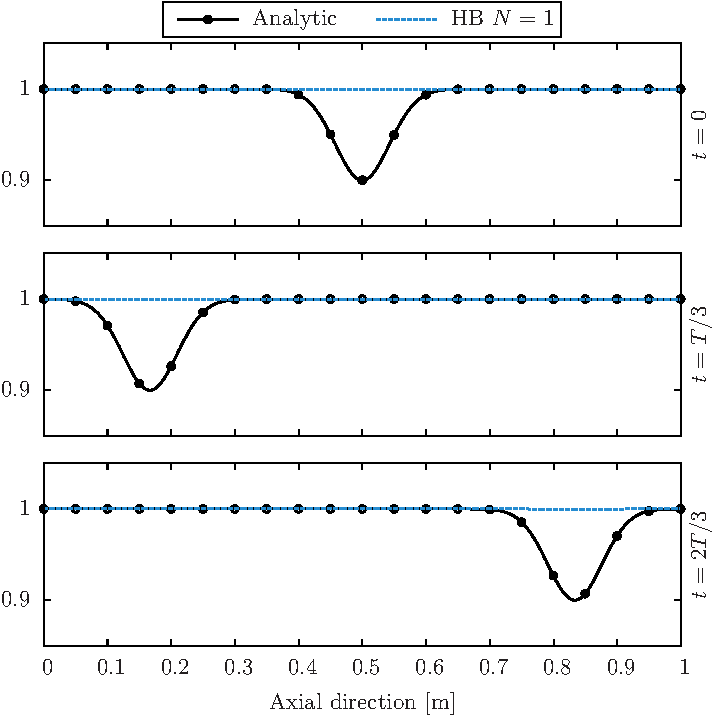
\includegraphics[width=.35\textwidth]{convection_wake_N1.pdf}}
  \subfigure[$N=2$ computation]{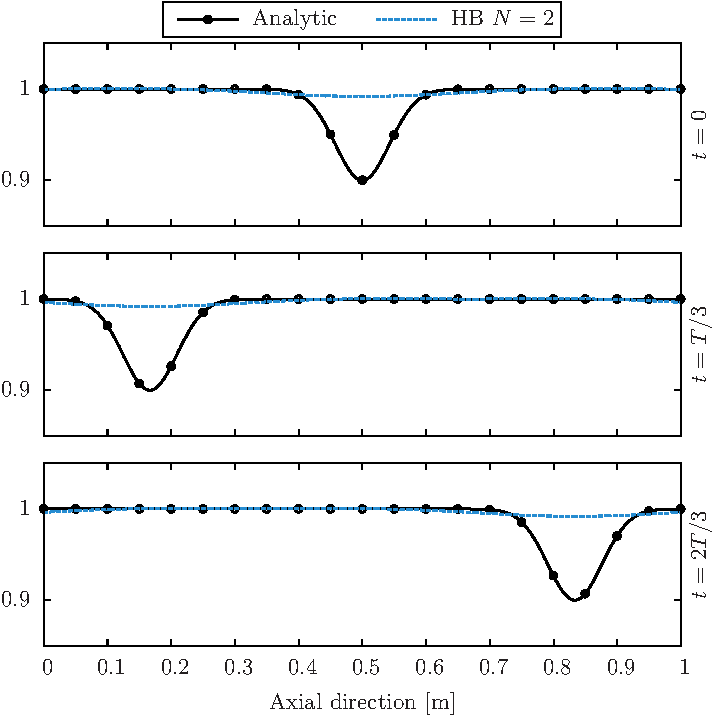
\includegraphics[width=.35\textwidth]{convection_wake_N2.pdf}}
  \subfigure[$N=3$ computation]{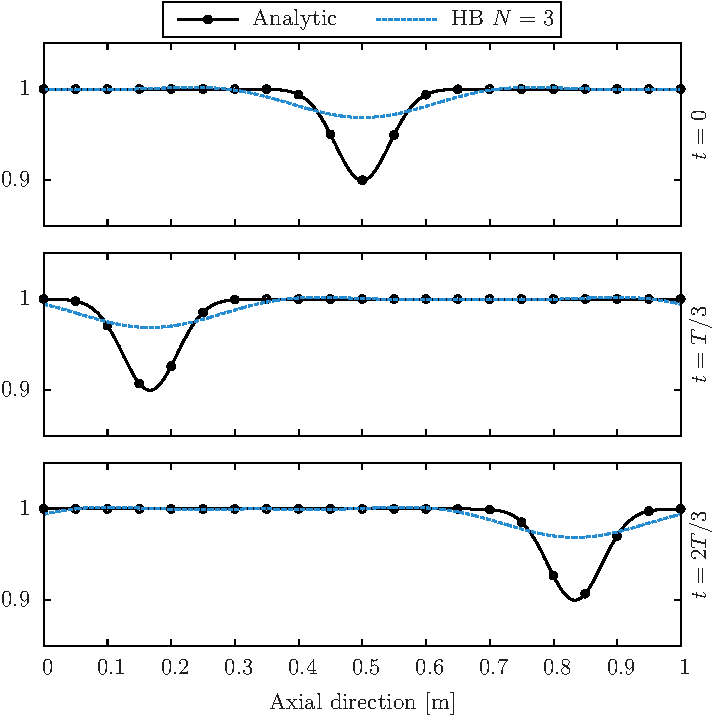
\includegraphics[width=.35\textwidth]{convection_wake_N3.pdf}}
  \subfigure[$N=4$ computation]{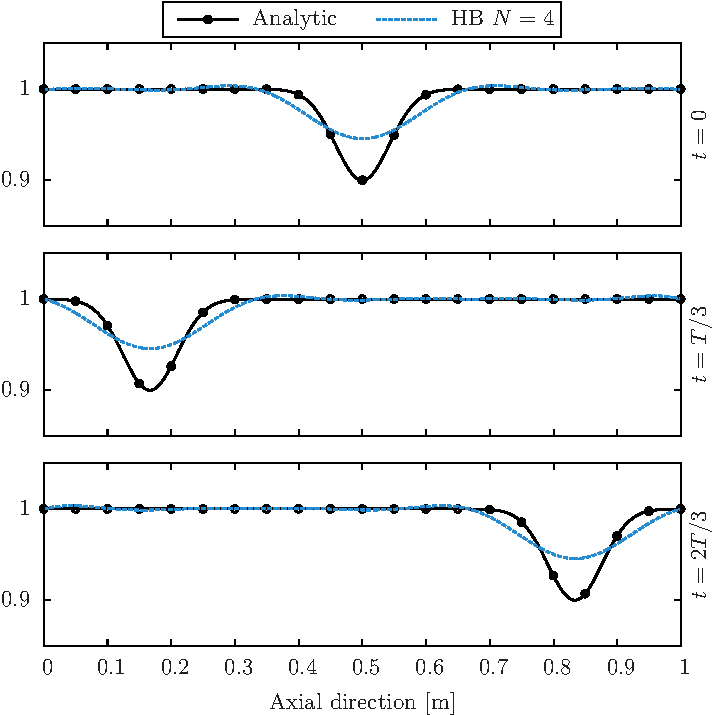
\includegraphics[width=.35\textwidth]{convection_wake_N4.pdf}}
  \subfigure[$N=5$ computation]{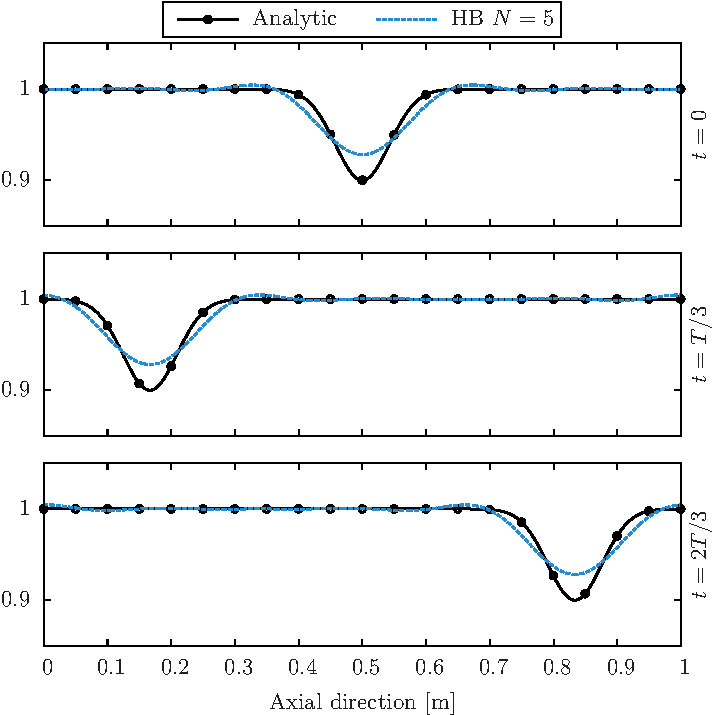
\includegraphics[width=.35\textwidth]{convection_wake_N5.pdf}}
  \subfigure[$N=6$ computation]{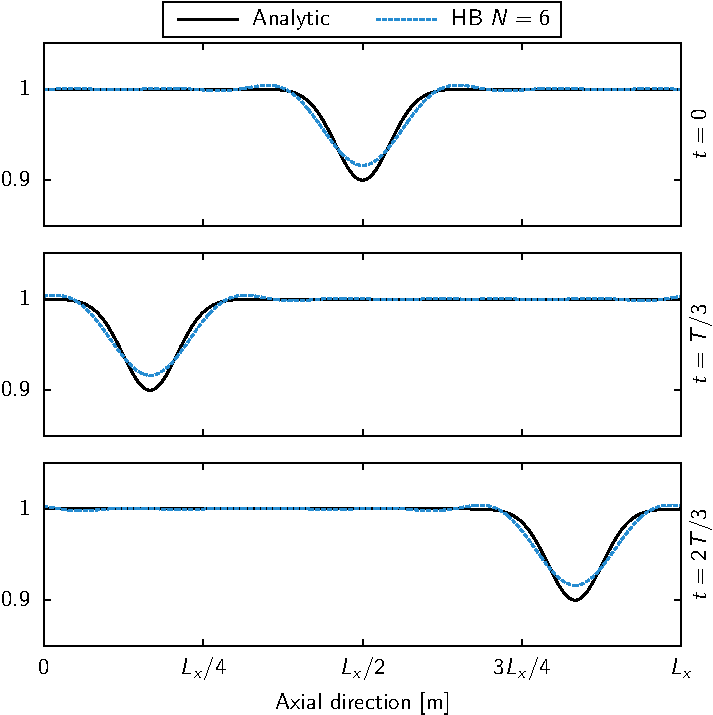
\includegraphics[width=.35\textwidth]{convection_wake_N6.pdf}}
  \caption{Harmonic balance results for 
  an injected Gaussian function representing a turbomachinery wake.}
  \label{fig:inj_wake_results}
\end{figure}
Figure~\ref{fig:inj_wake_results} depicts the harmonic balance
computations from $1$ to $6$ harmonics. The convergence toward
the Gaussian function is monotonic and is almost reached
for $N=6$ harmonics. When the number of harmonics is
too small, the width and the depth of the wake are badly estimated
by the method. Moreover, some slight oscillations outside the wake
can be observed, and these disappear along with the growth of the
number of harmonics.

\begin{figure}[htbp]
  \centering
  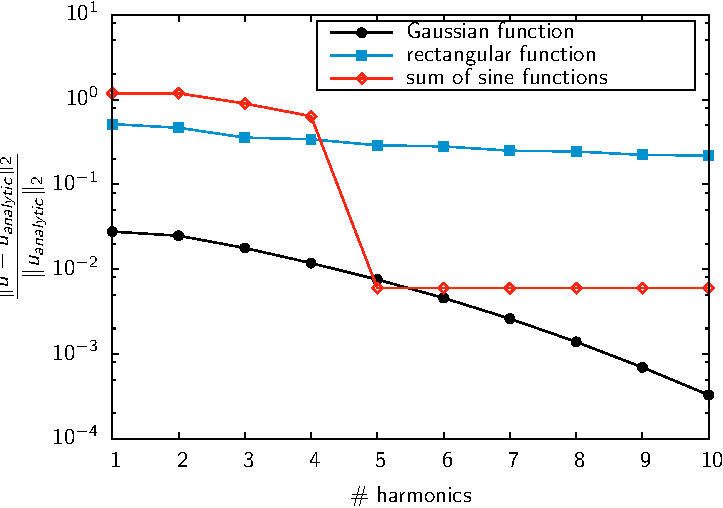
\includegraphics[width=.5\textwidth]{convection_wake_error.pdf}
  \caption{Convergence of the harmonic computations 
  for an injected Gaussian function representing a turbomachinery wake.}
  \label{fig:conv_wake}
\end{figure}
Figure~\ref{fig:conv_wake} shows the quantitative convergence of 
the harmonic balance computations for a Gaussian function. The
convergence for the two functions studied above are recalled
for comparison.
The convergence rate seams to follow an exponential function
and hence be better than the convergence of the rectangular function.
\begin{figure}[htbp]
  \centering
  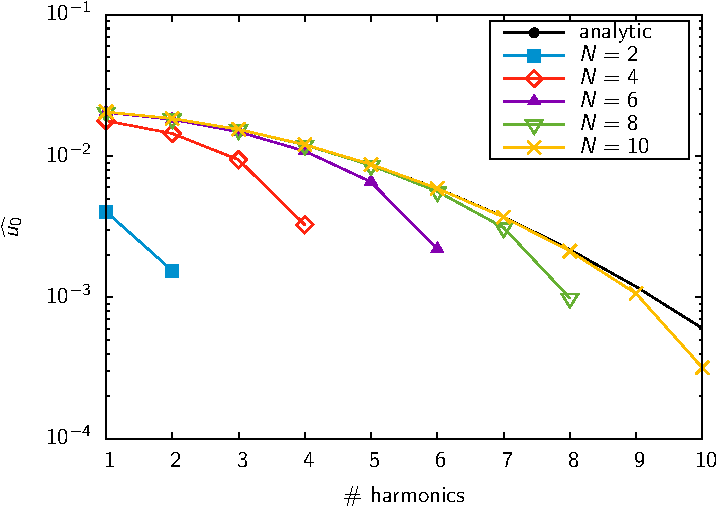
\includegraphics[width=.5\textwidth]{convection_wake_dft.pdf}
  \caption{Discrete Fourier transform of the computational
  results compared to the analytical one for an injected 
  Gaussian function.}
  \label{fig:dft_wake}
\end{figure}
The discrete Fourier transform of the results is
depicted against analytical result in Fig.~\ref{fig:dft_wake}.
The $N=2$ and $N=4$ computations badly capture their frequencies.
Starting from the  $N=6$ computation, some of the lower 
frequencies are correctly captured, the last harmonics being
always under-estimated.
Again, adding more harmonics to the harmonic balance
computations greatly improves the resolution of the
modes.

From the previous sections, one can conclude that for
Fourier-Based methods computations, no order
of convergence stands out. The convergence rate follows the decrease
of the spectrum of the temporal signal considered.
This can be named a spectral convergence.

Below some analytical considerations will help us
define a truncation error for the case of wake capturing.

\paragraph{Mathematical analysis of the Gaussian wake model}
\label{sec:analytical_considerations}

The Fourier transform of a Gaussian function is a Gaussian function itself.
If $g$ is a Gaussian function defined as:
\begin{equation}
    g(x) = A e^{-\alpha x^2},
    \label{eq:simple_gaussian_function}
\end{equation}
where $A$ and $\alpha$ are constants, then its Fourier transform is:
\begin{equation}
    \mathcal{F} [g(x)] = \mathcal{F} \left[A e^{-\alpha x^2} \right] = 
    A \sqrt{\frac{\pi}{\alpha}}
      e^{\frac{- \left( \pi f \right)^2}{\alpha}} = \widehat{g}(f),
    \label{eq:fourier_transform_gaussian}
\end{equation}
where $\mathcal{F}$ denotes the Fourier transform operator and $f$ the 
frequency.
$\widehat{g}$ can then be re-written as a classical Gaussian function:
\begin{equation}
    \widehat{g}(f) = A^\prime e^{-\alpha^\prime f^2},
    \label{eq:simple_gaussian_function_spectre}
\end{equation}
where:
\begin{equation}
  \begin{cases}
    A^\prime=A \sqrt{\frac{\pi}{\alpha}}\\
    \alpha^\prime = \frac{\pi^2}{\alpha}.
  \end{cases}
\end{equation}
The exponential factor of the wake law~$\alpha$ is inversely
proportional to its Fourier counter-part~$\alpha'$, meaning that their
width will vary in opposite way: the wider the wake, the thinner its
spectrum and vice-versa.

For the similarity law of Lakshminarayana and Davino, $\alpha$ and $\alpha^\prime$ can be identified:
\begin{equation}
    \alpha =  0.693 \left( \frac{2}{L} \right)^2, \quad
    \alpha^\prime =  \frac{1}{0.693} \left( \frac{\pi L}{2} \right)^2.
    \label{eq:gaussian_params_laksh}
\end{equation}

We have proven above that the convergence rate is inherently linked to
the spectrum of the considered unsteady signal.
As the spectrum of the wake is analytical here, one
way to define the theoretical truncation error is to consider 
the energy contained in the unresolved 
part of the spectrum divided by the energy of the full spectrum:
\begin{equation}
    \varepsilon_{th}(f) = \sqrt{\frac{
        \int_f^\infty | \widehat{g}(\zeta)|^2 d \zeta
      }{
        \int_0^\infty | \widehat{g}(\zeta)|^2 d \zeta
      }}.
    \label{eq:def_truncation_error}
\end{equation}
Introducing the error function defined as
\begin{equation}
    \erf(x) = \frac{2}{\sqrt{\pi}} \int_0^x e^{-t^2} dt,
\end{equation}
and the complementary error function defined as
\begin{equation}
    \erfc(x) = 1 - \erf(x) = \frac{2}{\sqrt{\pi}} \int_x^\infty e^{-t^2} dt,
\end{equation}
then
\begin{align}
    \int_0^\infty | \widehat{g}(\zeta)|^2 d \zeta 
    &= \frac{1}{2} \int_{- \infty}^\infty | \widehat{g}(\zeta)|^2 d \zeta \\
    &= \frac{A^{\prime 2}}{2} \sqrt{\frac{\pi}{2 \alpha^\prime}},
\end{align}
and
\begin{equation}
    \int_f^\infty | \widehat{g}(\zeta)|^2 d \zeta = 
      \frac{A^{\prime 2}}{2} \sqrt{\frac{\pi}{2 \alpha^\prime}} \erfc (\sqrt{2 \alpha^\prime} f).
\end{equation}

The theoretical truncation error can then be written as:
\begin{equation}
    \varepsilon_{th}(f) = \sqrt{\erfc (\sqrt{2 \alpha^\prime} f)}.
    \label{eq:analytical_conv}
\end{equation}
One can notice from Eq.~\eqref{eq:analytical_conv} that the 
truncation error does not depend on the wake deficit.

\begin{figure}[htb]
  \begin{center}
    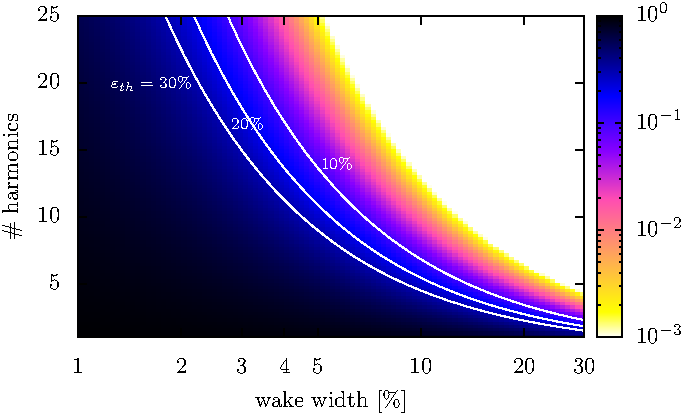
\includegraphics[width=.85\textwidth]{ANALYTICAL_ERROR_PPT.pdf}
  \end{center}
  \caption{Theoretical truncation error of the Lakshminarayana and Davino wake law.}
  \label{fig:analytic_error_paper}
\end{figure}
Eq.~\eqref{eq:analytical_conv} is depicted in
Fig.~\ref{fig:analytic_error_paper}. 
It can be seen that the wider the spectrum,
the higher the number of harmonics needed to
have a certain level of error. 
Moreover, for a thin wake width ($2 \%$ of the pitch)
the number of harmonics required to capture it with a truncation 
error of $10\%$ is up to $25$ harmonics
which states the limit for Fourier-based methods efficiency.
This figure is analytical meaning that it can give an idea
of the number of harmonics required to compute a wake of a given width.
In the previous section, the wake analyzed had a width
of $10\%$. According to the analytical Eq.~\eqref{eq:analytical_conv},
a $10\%$ error is achieve by using $N=7$ harmonics.

The next section details the convergence obtained with Fourier-based methods
on a reduce order problem: two rotating blocks are considered with
a Lakshminarayana and Davino wake injection.

\section{Solution: towards a prediction tool}
\label{sec:CROR}

Originally, this study has been done to understand the convergence
issues seen on Contra-Rotating Open Rotors (CROR) configurations.
In contrast to turbomachinery applications, convergence
in terms of harmonics has been observed to be
slow on some configurations. For instance, computations
made on the \aipx CROR
are still not converged at $N=10$ harmonics.
Conversely, convergence is obtained at $N=7$ harmonics
for the \mockup configuration at high-speed as shown in
Fig.~\ref{fig:cptsm}.
\begin{figure}[htb]
  \centering
  \subfigure[high-speed \aipx computed with $N=10$ harmonics]{
    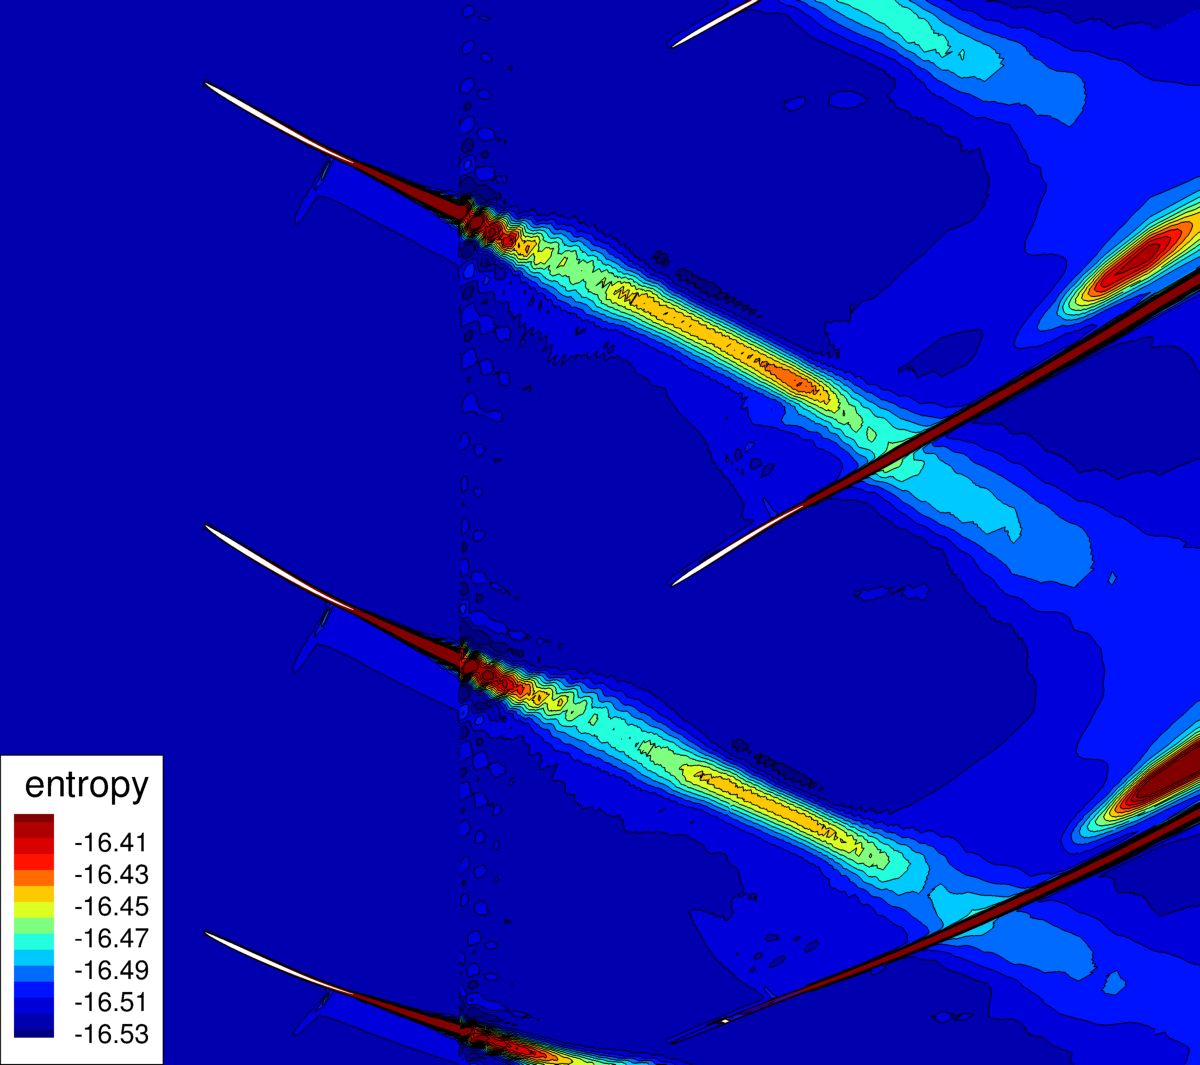
\includegraphics[width=.4\textwidth]{aipx7_entropy_r75_N10.jpg}
    \label{fig:cptsm_1}}\quad
  \subfigure[high-speed \mockup computed with $N=7$ harmonics]{
    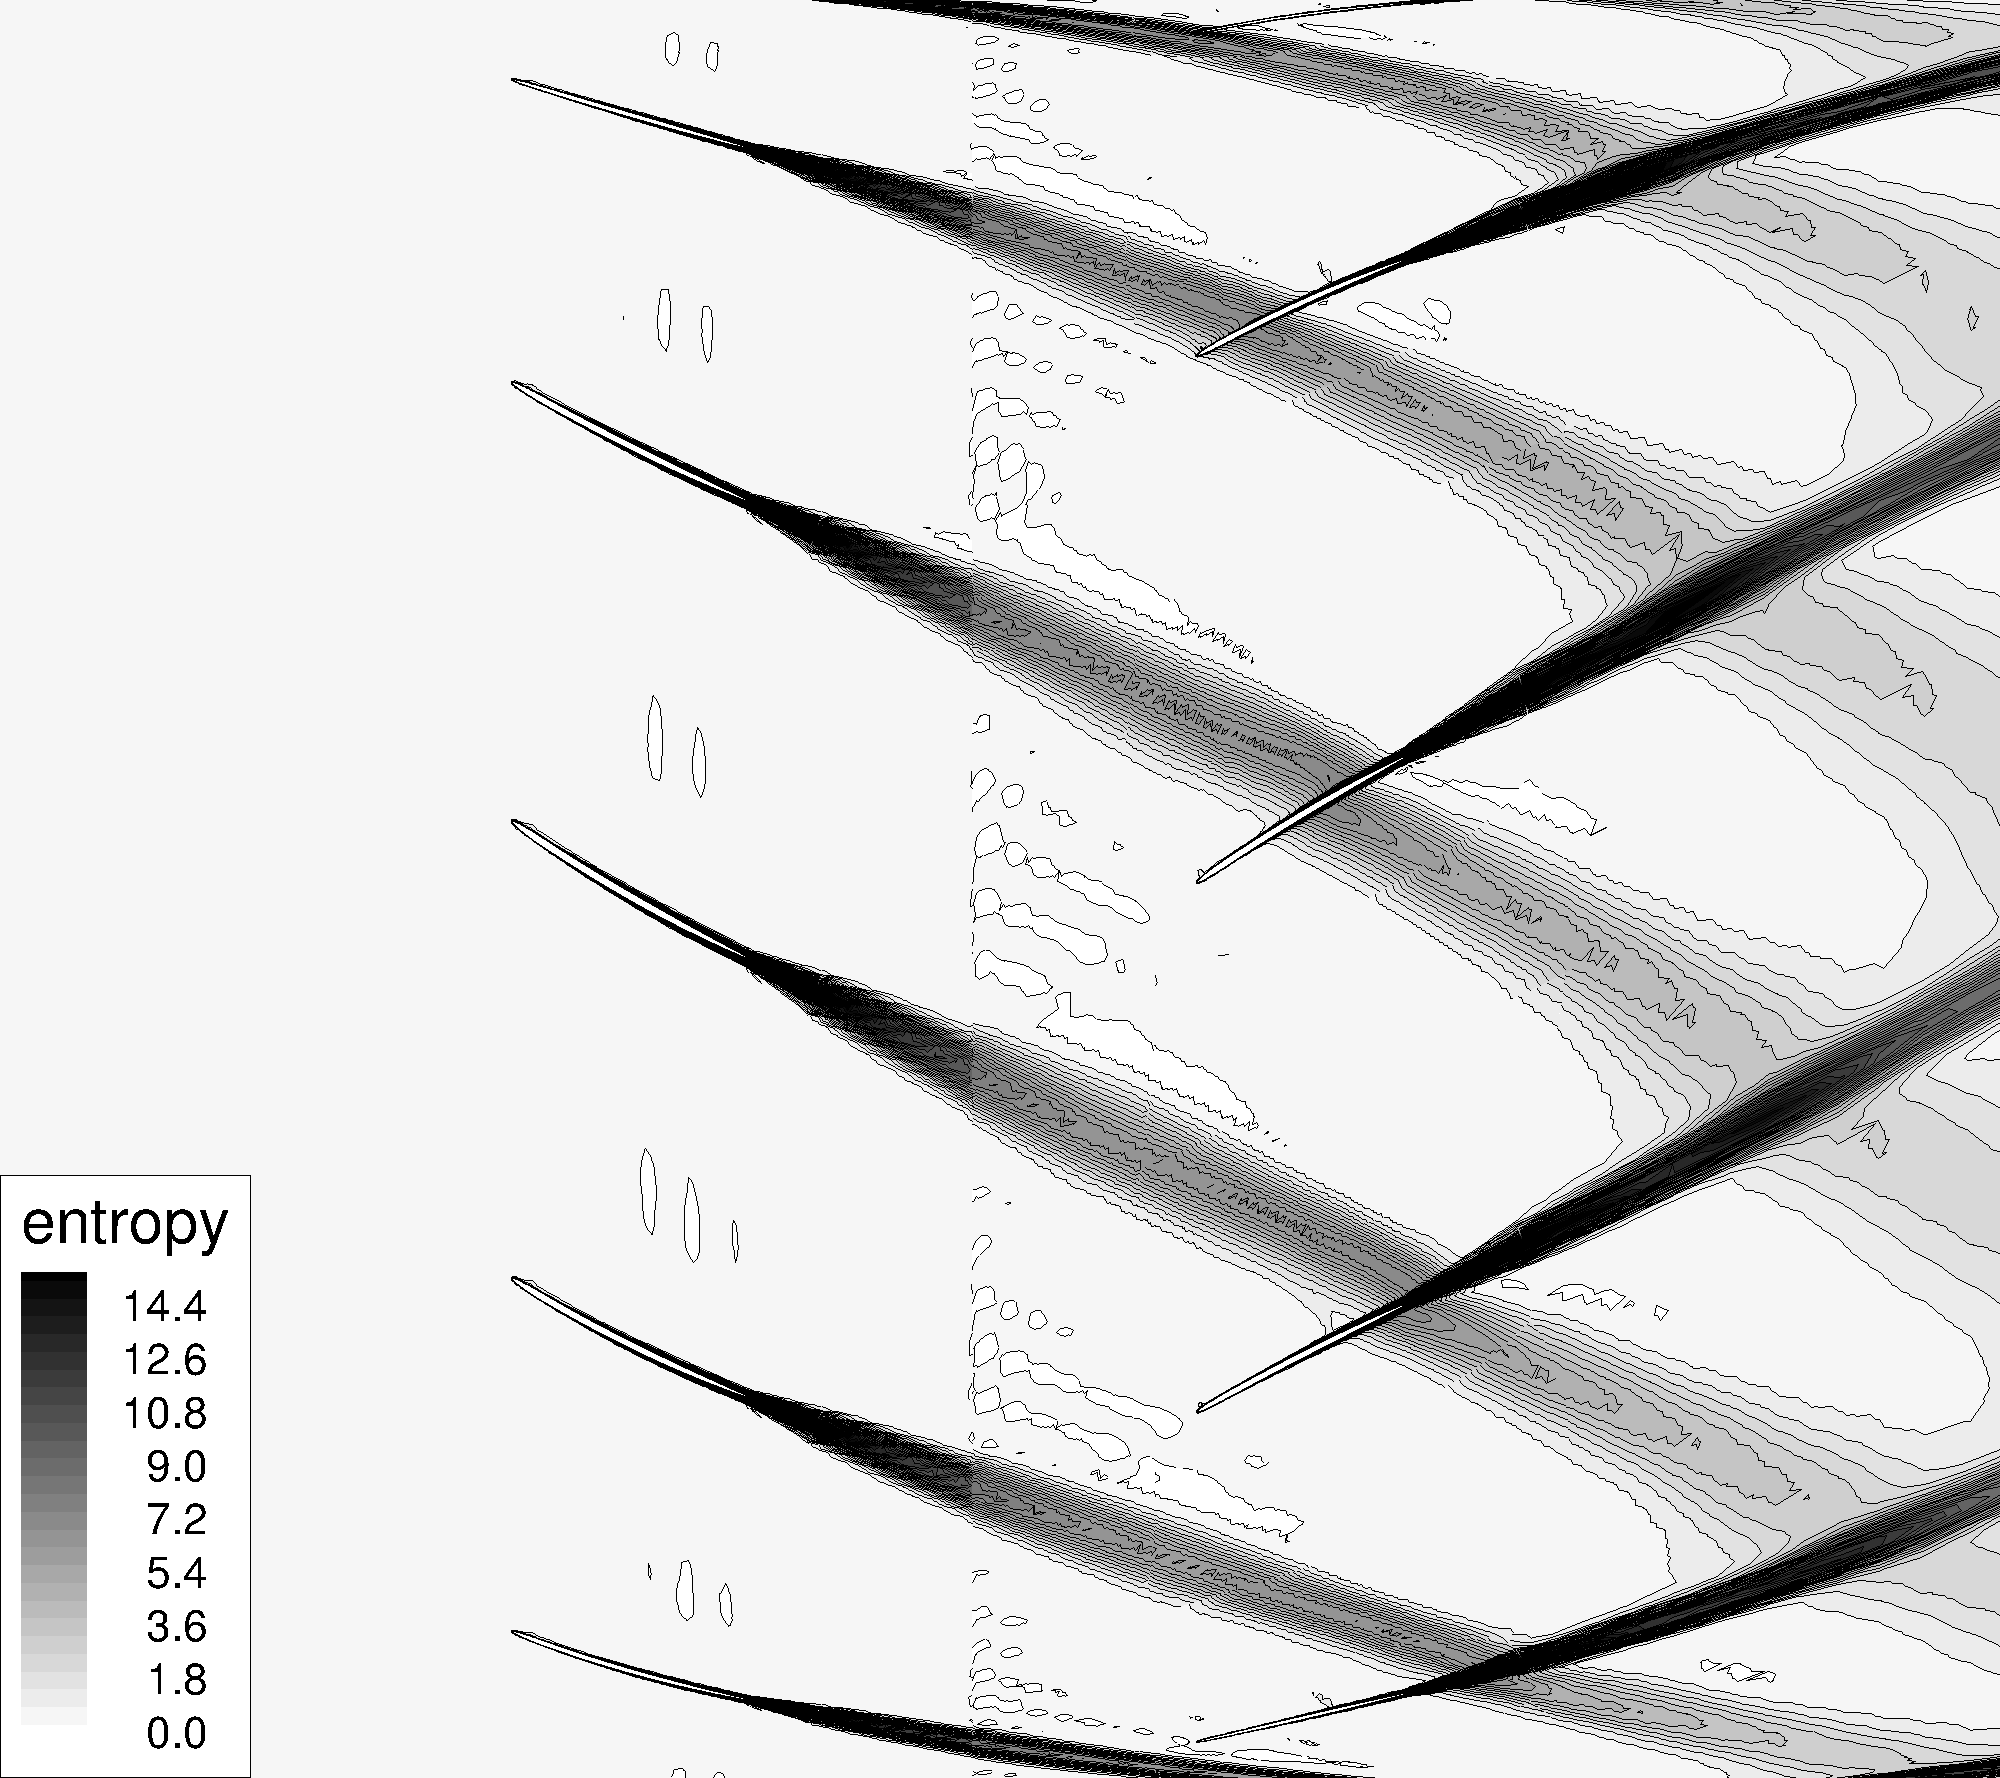
\includegraphics[width=.4\textwidth]{DREAM_HS_TSM_N7_roe3_sa_slice_r_75_entropy_BW.png}
    \label{fig:cptsm_2}}
  \caption{Entropy field of harmonic balance computation 
  for two CROR configurations at $75\%$ relative span.}
  \label{fig:cptsm}
\end{figure}
To investigate this issue, three configurations are studied:
\begin{itemize}
  \item the \aipx CROR 
  at high-speed (or cruise) condition
  and flight level (\emph{i.e.}  $P_i=23,842$~Pa and $T_i=219.6$~K),
  \item the \mockup CROR at low and high-speed conditions
  but at ground level (\emph{i.e.} $P_i=101,300$~Pa and
  $T_i=293$~K). In fact, these two cases were prone to 
  experimental investigations, hence the ground level.
\end{itemize}
Initially, it has been discovered that adding more harmonics in
the HB computations results in the improvement
of the capture of the wake.
Fig.~\ref{fig:crorroxvmap} shows the
axial momentum taken at the rotor/rotor interface
for the three considered configurations. These are extracted
from an affordable mixing-plane computation~\cite{Denton1979}.
It can be seen that, upstream the rotor-rotor interface,
the main tangential distortion seen is the wake. 
This is true for 
a relative span between $10\%$ and $90\%$, where $0\%$ corresponds
to the hub and $100\%$ the blade tip. 
For higher relative span, the distortion that is seen
is attributed to the tip-vortex, while smaller
relative span highlights viscosity effects near the hub.
One can observe different wake shapes. The High-Speed (HS) \aipx wake looks much
thinner than the HS \mockup which also looks
thinner than the Low-Speed (LS) one. Indeed, the latter does not show a
well delimited wake structure all along the span.
\begin{figure}[htbp]
  \centering
  \subfigure[\mockup -- low speed]{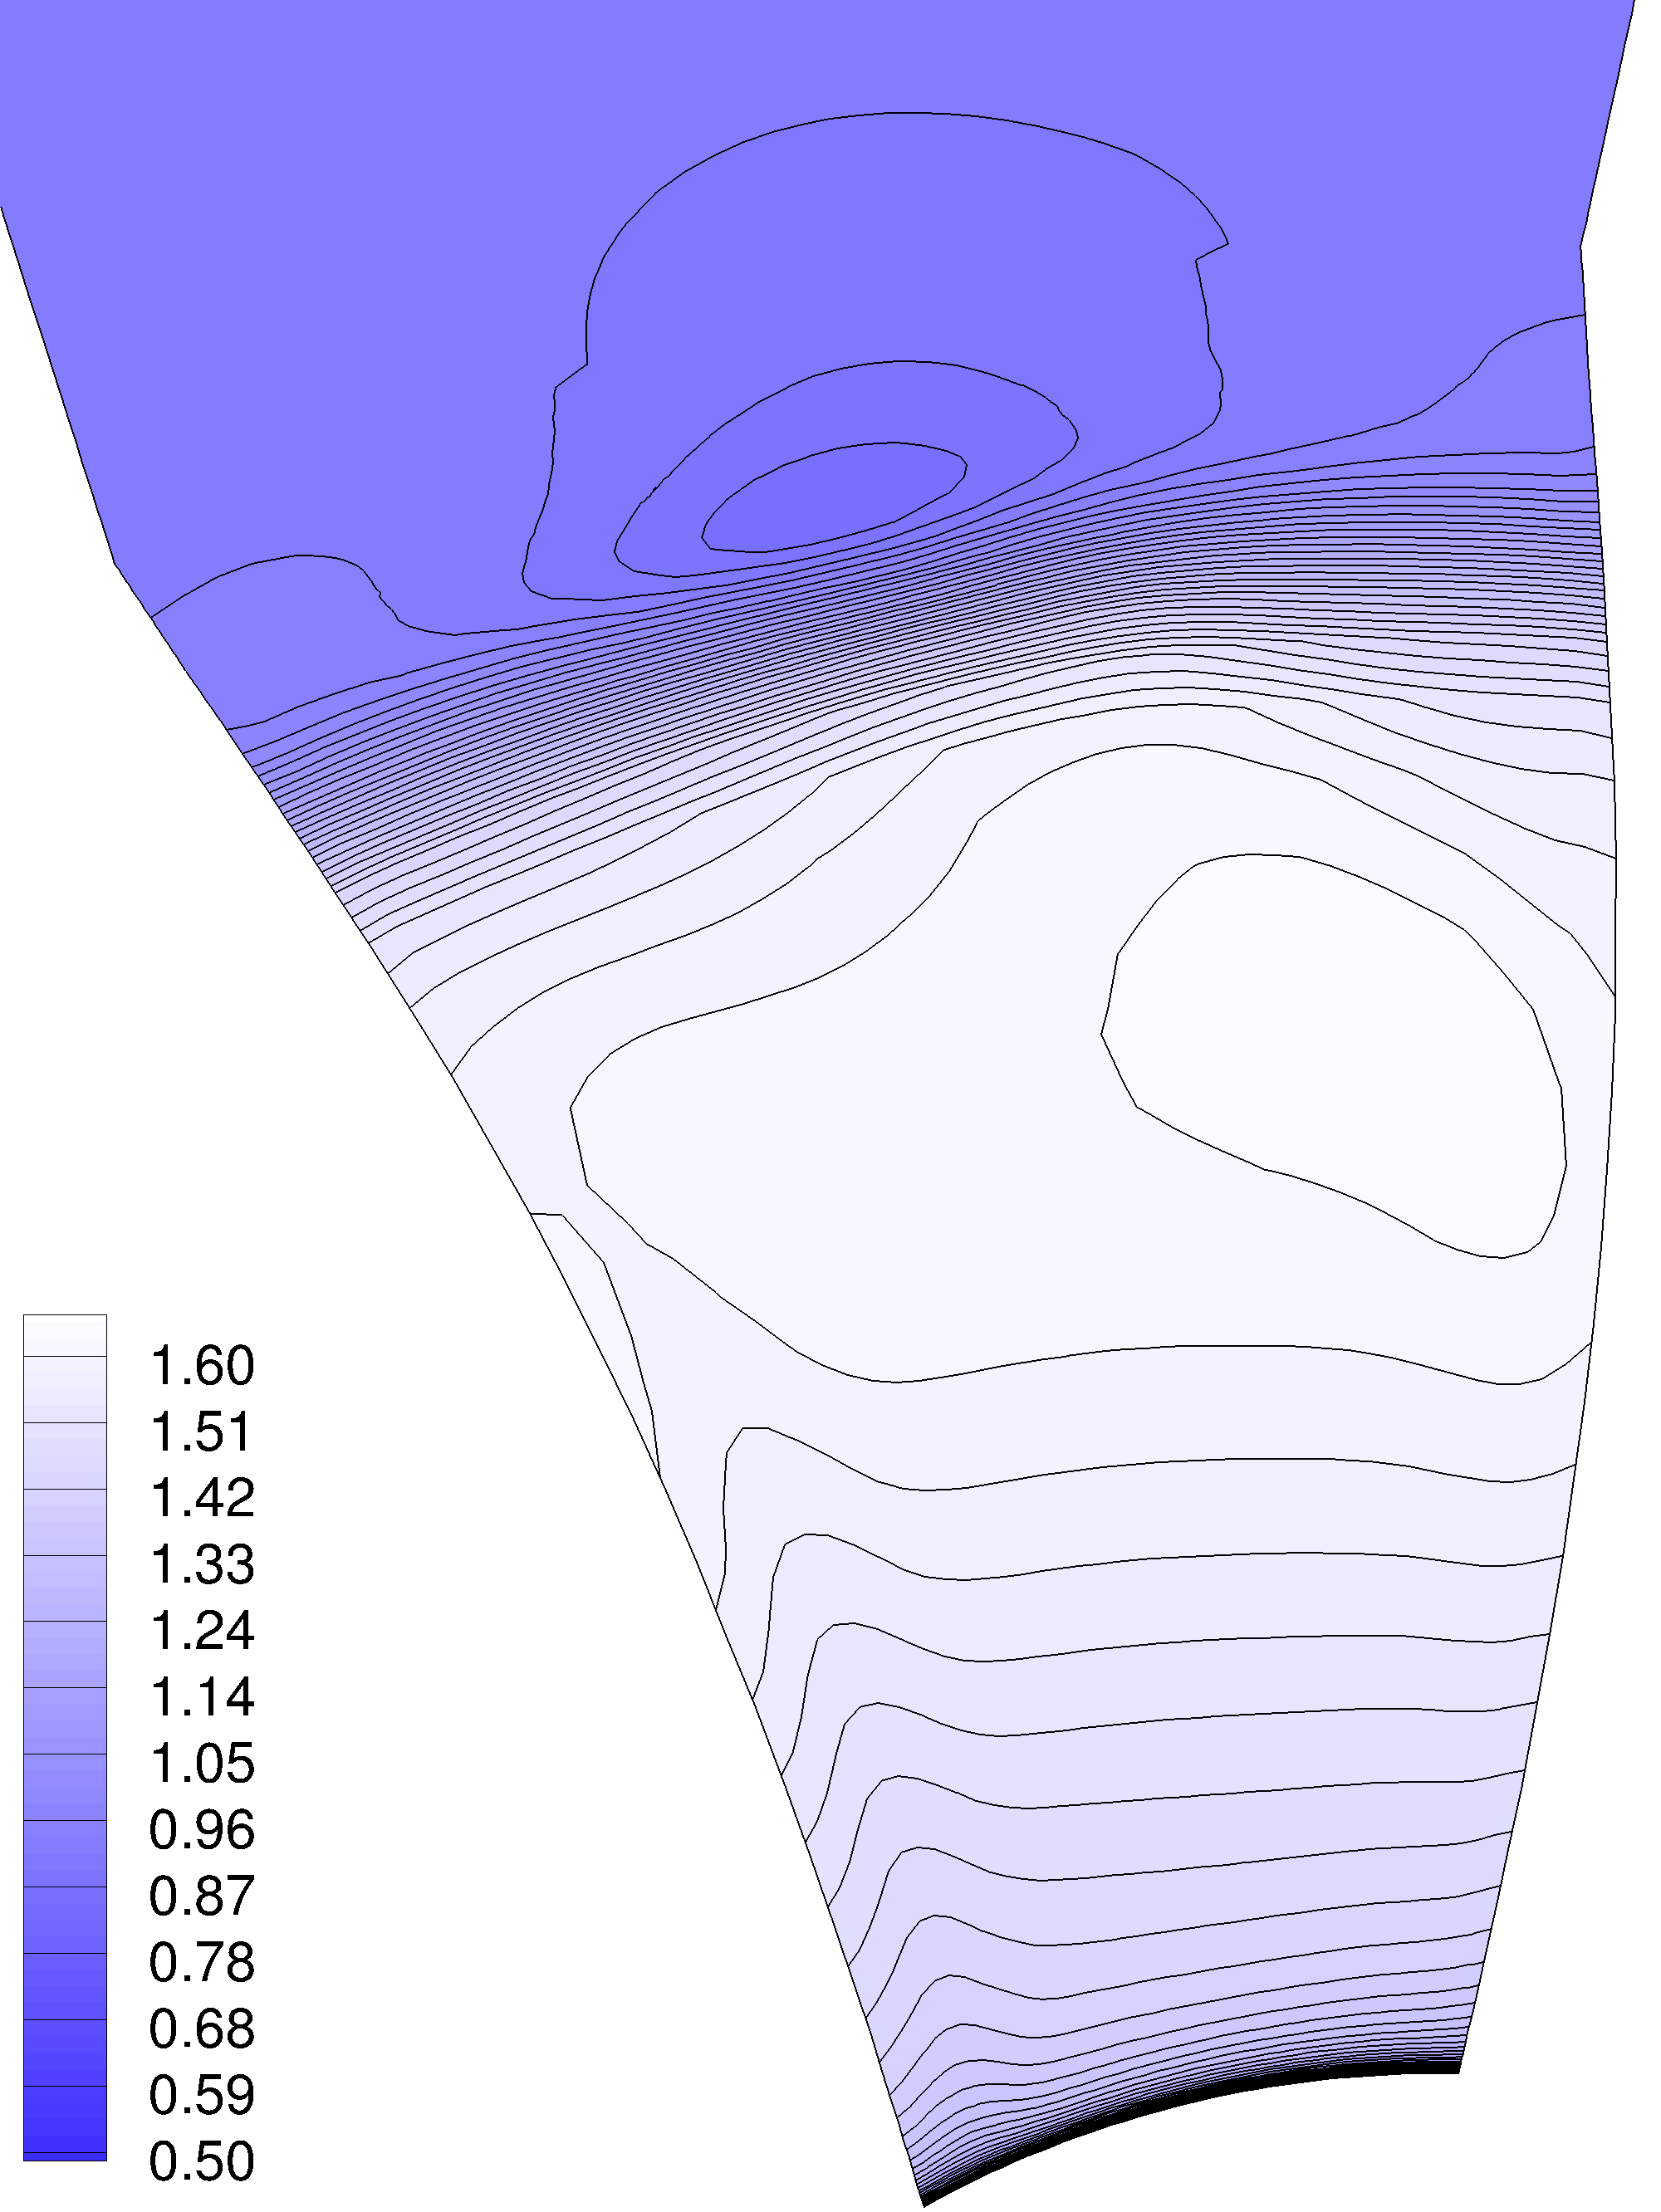
\includegraphics[width=.32\textwidth]{dream_ls.png}}
  \subfigure[\mockup -- high speed]{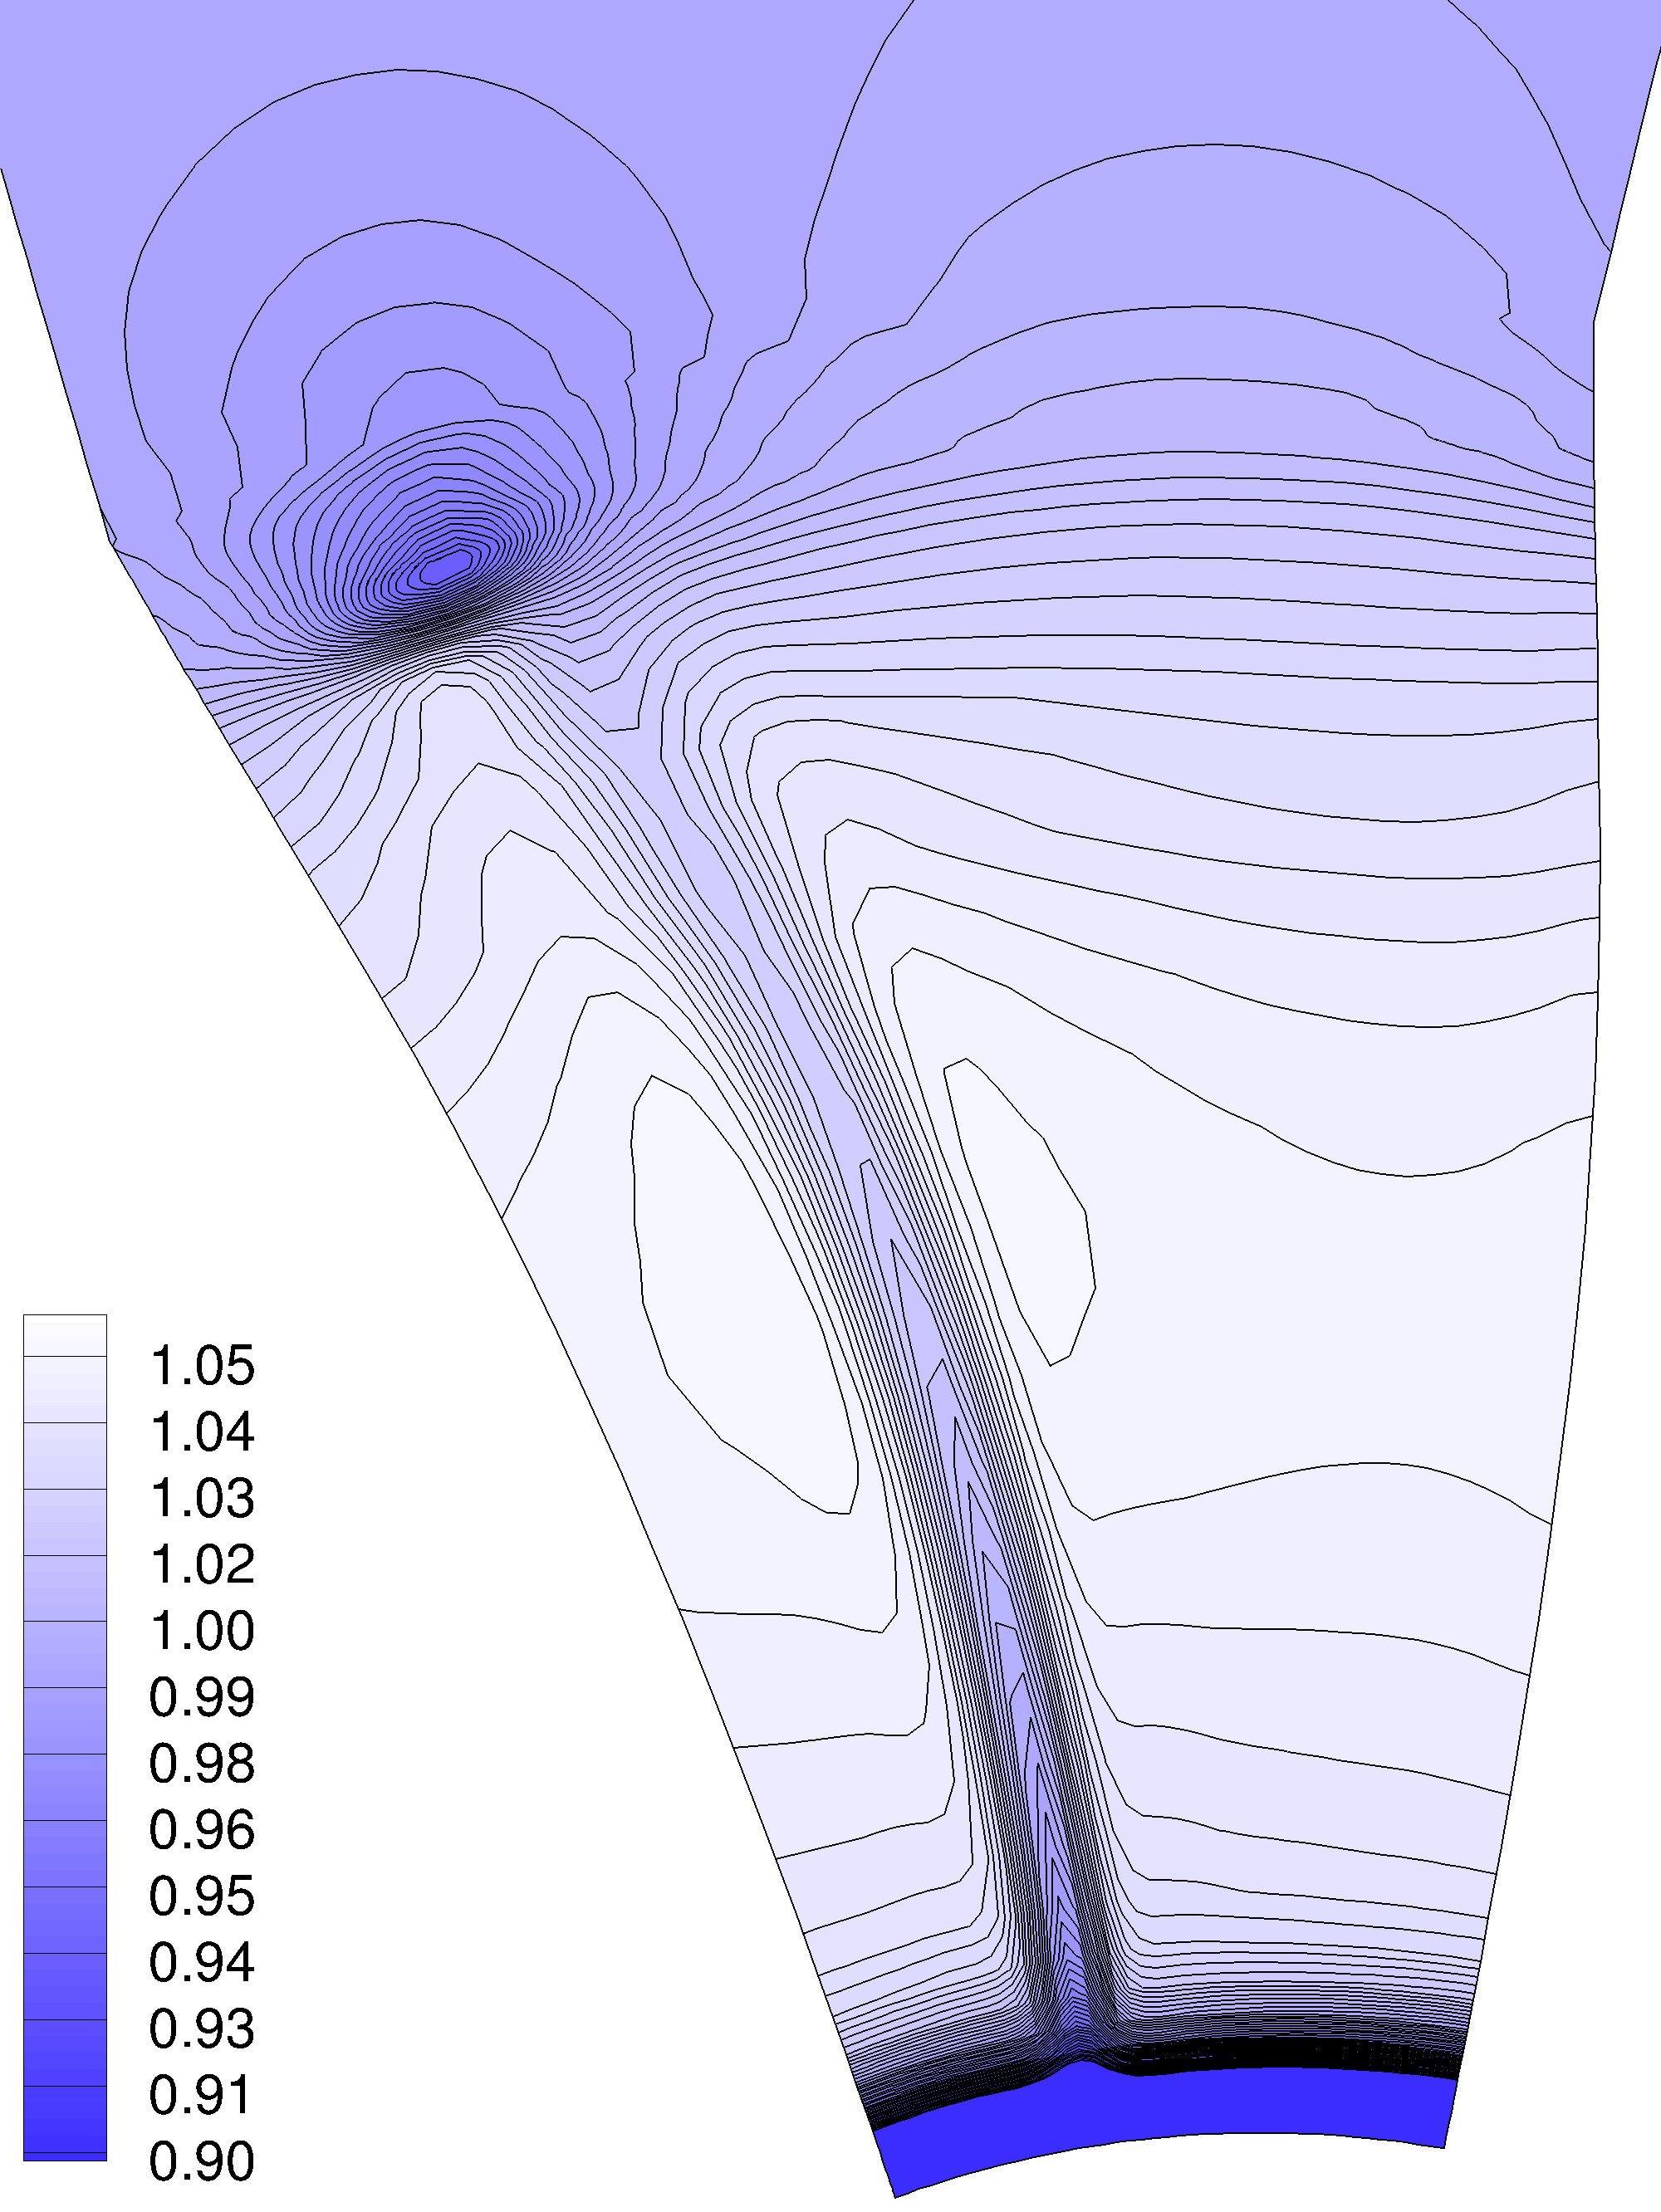
\includegraphics[width=.32\textwidth]{dream_hs_roe2.png}}
  \subfigure[\aipx -- high speed]{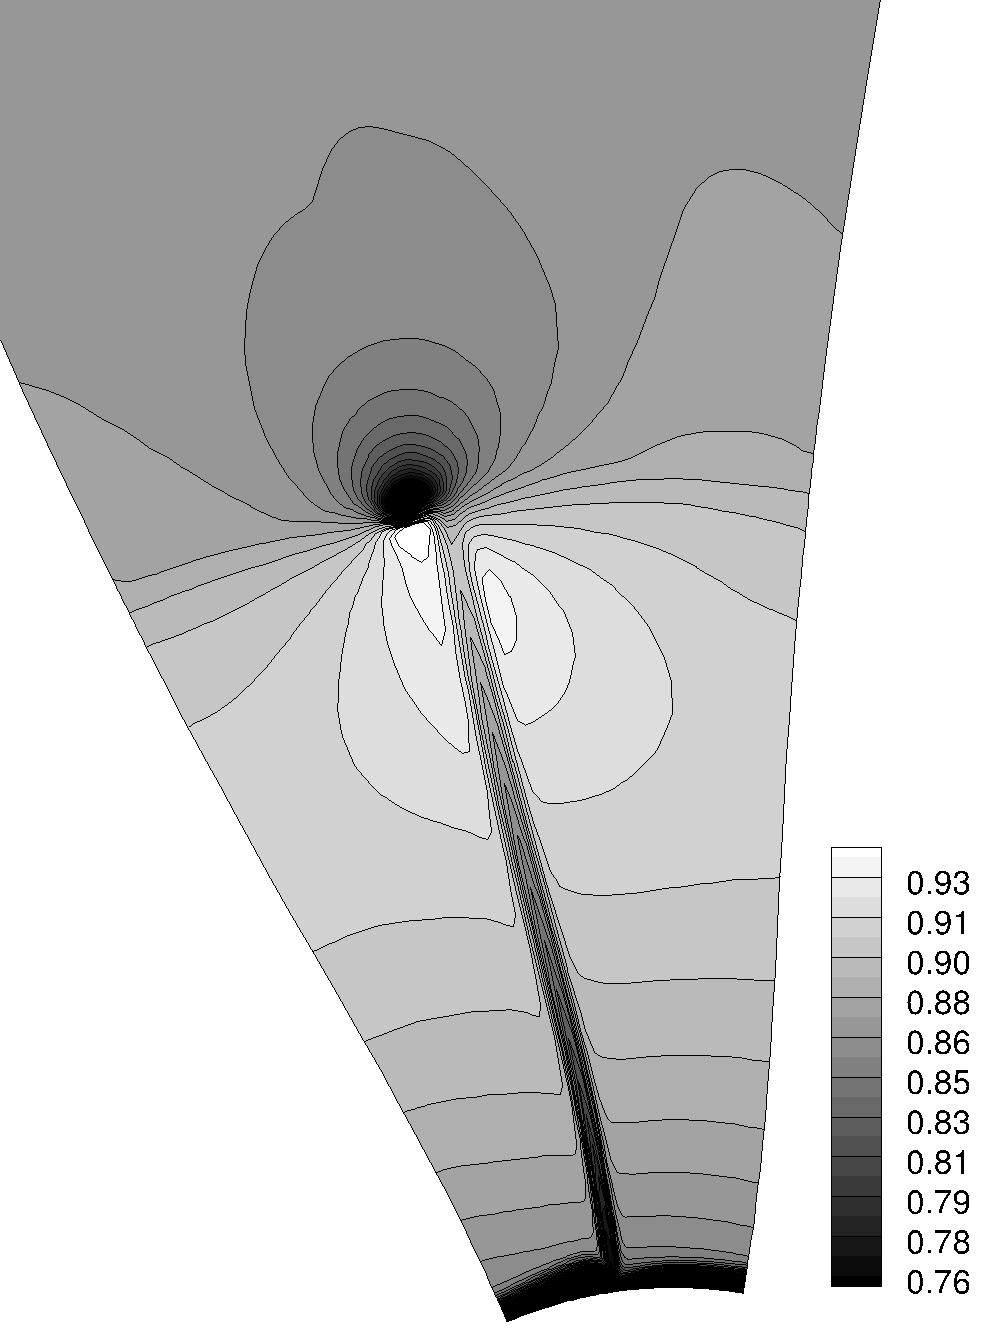
\includegraphics[width=.32\textwidth]{aipx7.png}}
  \caption{Non-dimensional axial momentum $(\rho U)/(\rho U)_\infty$ 
  upstream the rotor/rotor interface.}
  \label{fig:crorroxvmap}
\end{figure}

\subsection{Wake width criterion}
At first order, one can thus infer that for a relative
span contained between $10\%$ and $90\%$, the main
tangential distortion seen is the wake. 
To estimate the wake thickness, a curve
fitting algorithm is used to fit the Lakshminarayana
and Davino Gaussian wake law. The thickness
of the wake is plotted in Fig.~\ref{fig:crorwakethick_a}.
\begin{figure}[htbp]
  \centering
  \subfigure[Thickness estimation]{
  \label{fig:crorwakethick_a}
  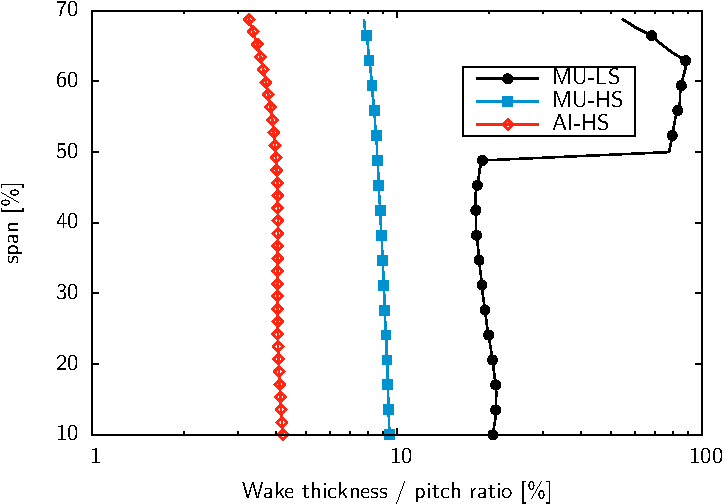
\includegraphics[width=.45\textwidth]{CROR_THICKNESS.pdf}}
  \subfigure[$\mathcal{L}2$-norm for the estimation]{
  \label{fig:crorwakethick_b}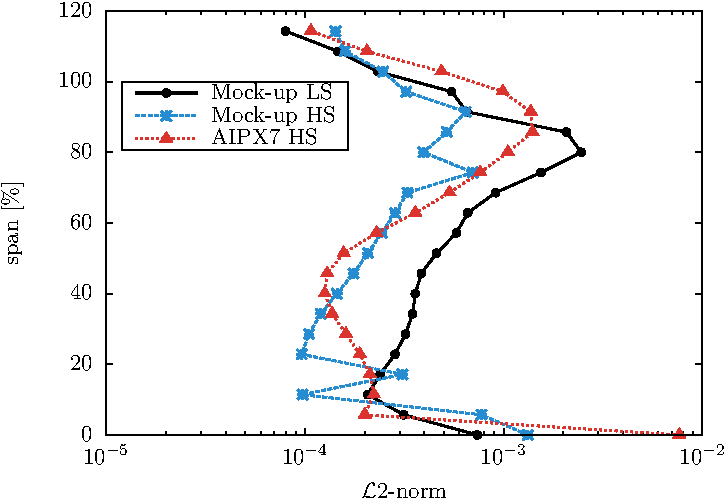
\includegraphics[width=.45\textwidth]{CROR_THICKNESS_ERROR.pdf}}
  \caption{Estimation of the relative wake thickness for the three contra-rotating
  open rotor configurations.}
  \label{fig:crorwakethick}
\end{figure}
To assess the quality of the curve fitting
algorithm, the $\mathcal{L}2$-norm
of the error is plotted in Fig.~\ref{fig:crorwakethick_b}.
For all three configurations, the error follows the same trend.
Near the hub (relative span inferior to $10\%$) the error is
maximum. Between $10\%$ and $70\%$ the error increases but
remains relatively low. This is the region
where the main tangential distortion is
actually a wake, hence the good fitting. 
In the tip vortex region (relative
span between $70\%$ and $100\%$), the error increases
and reaches a maximum in the core of the tip vortex.
In this region, the tangential distortion is not a wake
and explains the difficulty of the curve fitting algorithm
to capture a Gaussian function.
Finally, in the far-field region (relative span superior to $100\%$)
the axial momentum decreases toward the infinite velocity, thus
the tangential distortion is a constant field, which explains
the low error.
To qualitatively estimate the level of the curve fitting,
the best (from \mockup HS configuration) and the
worst fits (from \mockup LS CROR) are compared to their
original wake signals in Fig.~\ref{fig:crorwakeestimate}.
For the best fit, the original tangential distortion is
almost superimposed on the equivalent Gaussian wake law, besides
the fact that the wake is not symmetrical. In opposite,
the tangential distortion seen for the worst fit looks like
an inverse Lakshminarayana and Davino wake and does not  
\begin{figure}[htbp]
  \centering
  \subfigure[Best fit]{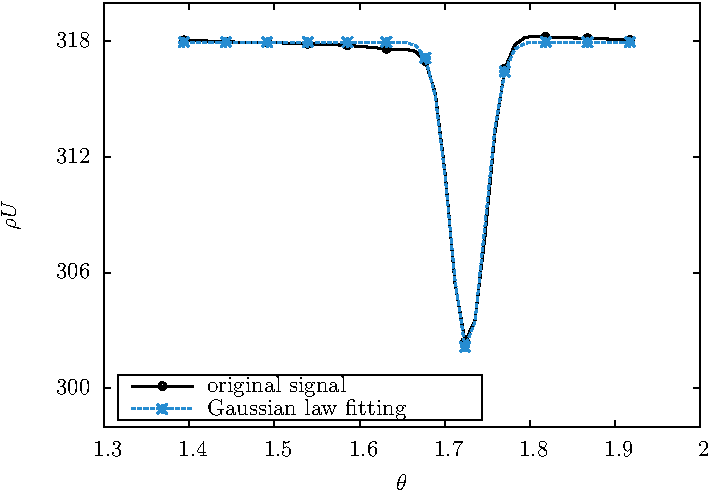
\includegraphics[width=.45\textwidth]{CROR_WAKE_FITTING_BEST.pdf}}
  \subfigure[Worst fit]{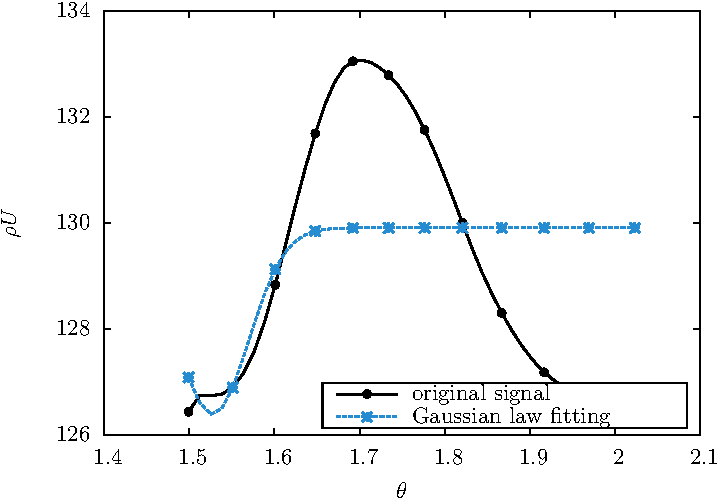
\includegraphics[width=.45\textwidth]{CROR_WAKE_FITTING_WORST.pdf}}
  \caption{Qualitative estimation of the level of the curve fitting for the
  wake in CROR configurations.}
  \label{fig:crorwakeestimate}
\end{figure}
From the error estimate (Fig.~\ref{fig:crorwakethick_b})
and the best/worst fit scenario, one can deduce that
curve fitting works well when the distortion is a wake.
In that case, the thickness estimation is reliable. 

One can thus say that the wake is relatively well-defined
between $10\%$ and $70\%$ relative span. 
It can be seen that the wake of the 
LS \mockup is about $30\%$ of the pitch, the one of the HS
\mockup 
being approximately $10\%$ while the
\aipx wake is thinner as it is around $4\%$ of the pitch.

Based on the
analytical formula derived in Sec.~\ref{sec:analytical_considerations},
if the wake width is known, one can deduce the
number of harmonics needed to capture a wished level of error
$\overline{\varepsilon}$:
\begin{equation}
    N = \frac{\ierfc \left[\overline{\varepsilon}^2 \right]}{
    \sqrt{2 \alpha^\prime}},
    \label{eq:estimation_nb_harms}
\end{equation}
where $N$ is the number of harmonics, $\ierfc$ the inverse 
complementary error function (namely $\erfc^{-1} = \ierfc$),
$\varepsilon$ and $\alpha^\prime$ are the truncation error
and the wake parameter, respectively, as defined in 
Sec.~\ref{sec:analytical_considerations}.
The level of error required 
for a computation to be rigorously converged
is difficult to estimate. 
Instead of using the level of error, 
we will use the
relative accumulated energy $E(f)$ as defined in 
Eq.~\eqref{eq:correspond_E_error}.
It seems reasonable, from an engineering standpoint, to consider
that a $99\%$ accumulation of energy should be a good starting point.
To emphasize that,
the reconstruction of a wake in function of three levels of cumulative
energy $E$ is depicted in Fig.~\ref{fig:level_of_energy}. 
\begin{figure}[htbp]
  \centering
  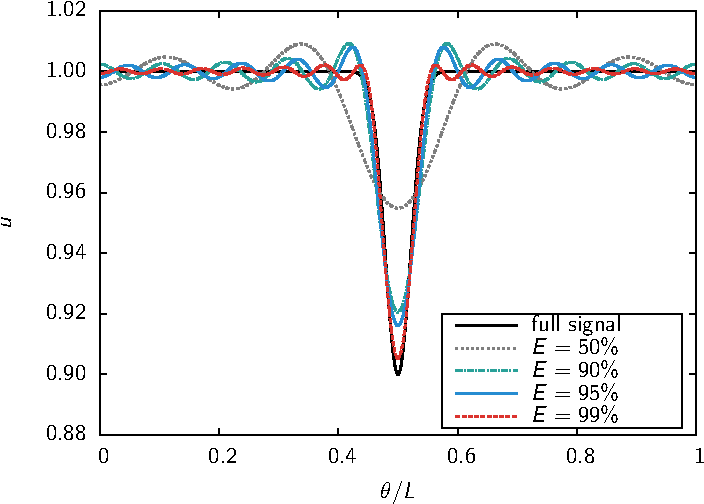
\includegraphics[width=.5\textwidth]{LEVEL_OF_ENERGY_PAPER.pdf}
  \caption{Reconstructions of a wake depending on
  the energy content kept in the signal.}
  \label{fig:level_of_energy}
\end{figure}
One can see
that a reconstruction using only $50\%$ of the energy
leads to a signal that has neither
the right wake deficit nor its width. Using
$90\%$ and $95\%$ of the energy improves things a little
but is still not satisfactory as large secondary
oscillations remains as long with a bad capture
of the wake deficit.
In opposite, by using $99\%$ of the energy to reconstruct
the signal, some extra
oscillations are seen but 
the wake width and deficit are recovered with less than 
$95\%$ accuracy.
Thus, the $99\%$ energy threshold ensures that the wake
will be correctly transmitted in the opposite row, which is
the prior concern of this paper.
Thus, based on the $99\%$ energy threshold
and the wake width computed
for all the three CROR configurations shown in Fig.~\ref{fig:crorwakethick},
one can estimate the number of harmonics needed to compute such
applications using Eq.~\eqref{eq:estimation_nb_harms}. 
Approximately, the wake width
of the \aipx, the HS \mockup and the LS \mockup is respectively
$4\%$, $10\%$ and $30\%$. 
Using Eq.~\eqref{eq:estimation_nb_harms},
the theoretical estimation of the number of harmonics needed 
to recover $99\%$ of the energy is respectively
$17$, $7$ and $2$. These numbers explain why the 
\aipx configuration is still not converged after $N=10$
harmonics. Moreover, such a computation leads to a
$87\%$ energy signal. Fig.~\ref{fig:level_of_energy}
supports the argument that with this level of energy, the wake
is not properly captured as a $90\%$ energy signal
does not accurately estimate the wake deficit and thickness.

With this approach, one can deduce approximately
the number of harmonics needed to compute such CROR
configurations using Fourier-based methods. The issue is that it is limited to
well defined wakes. If another tangential
distortion is seen at the interface, the present
criterion cannot be used, which limits the current
method. However, as demonstrated in Sec.~\ref{sub:comp_w_analytic},
the analytical error and the error based on an
azimuthal Fourier transform of the distortion
seen just upstream the interface for a mixing-plane
configuration are similar. 


\subsection{Prediction tool based on an azimuthal Fourier transform}
Thus, a more general way to analyze the spectrum in a wake is
to perform an azimuthal Fourier transform at the rows interface
in a mixing-plane computation. The good thing is
that it both encompass the wake analysis done above and also
any tangential disturbances as for instance
the viscosity effects near the hub or the tip vortex.
The steps to do such an analysis are detailed in
Fig.~\ref{fig:criterion_cror}. First the row
interface is extracted from a mixing-plane computation 
(step \textcircled{\small{$1$}}).
The term row is used to show that this can be done
for a CROR configuration and in general any turbomachinery
configuration where a relative speed motion exists at
the row interface.
The axial momentum is then extracted for a large
number of radii spanning the region of interest
(step \textcircled{\small{$2$}}).
In a CROR configuration this is the region with a 
relative span ranging between $0\%$ and $120\%$.
In fact, for higher relative span ($\geq 120\%$), the fluid motion
is not of prior interest as it is the far-field region.
Finally, for each radii, an azimuthal Fourier transform
is performed to obtain the tangential spectrum of the
axial momentum (step \textcircled{\small{$3$}}).
\begin{figure}[htbp]
  \centering
  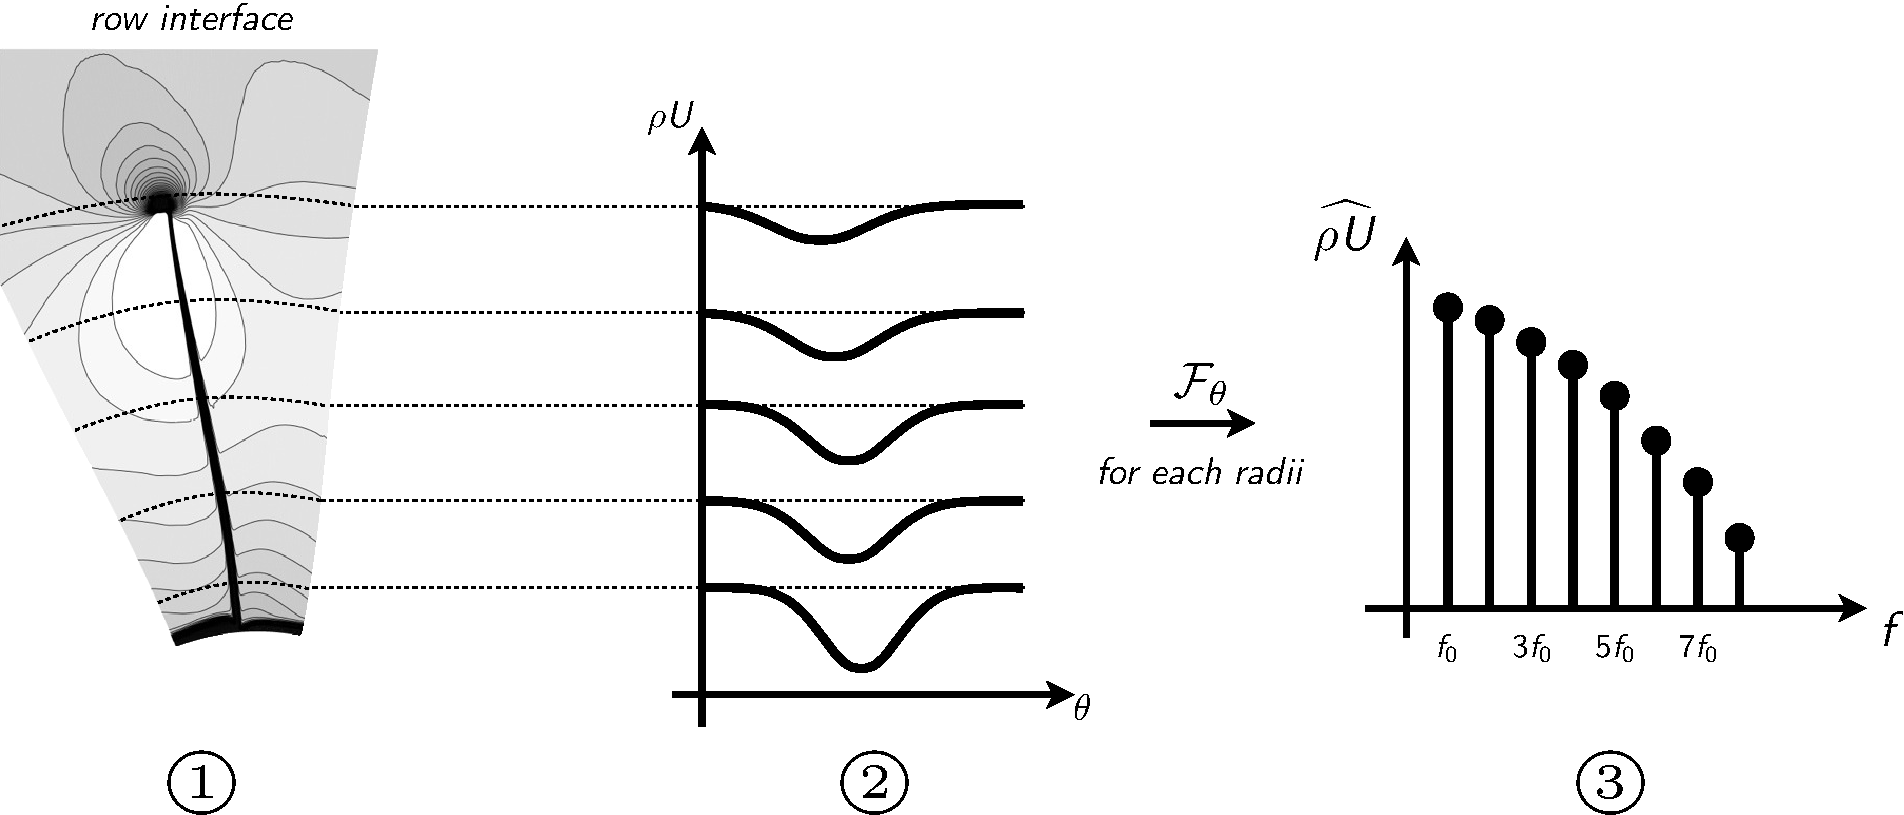
\includegraphics[width=.6\textwidth]{CRITERION_CROR.pdf}
  \caption{Steps for the prediction tool based on an azimuthal
  Fourier transform of the rotor-rotor interface.}
  \label{fig:criterion_cror}
\end{figure}
The relative cumulative energy is then easily defined as:
\begin{equation}
    E (N) = \frac{\sum_{k=1}^N \left[ \widehat{\rho U}^{\theta} (k) \right]^2}{ 
    \sum_{k=1}^\infty \left[ \widehat{\rho U}^{\theta} (k) \right]^2},
    \label{eq:def_crit_cror}
\end{equation} 
where $\widehat{\rho U}^{\theta}$ denotes the axial momentum spectrum
extracted from the rows interface plane. In Eq.~\eqref{eq:def_crit_cror},
the cumulative energy up to harmonic $N$ is 
compared to the total energy.
Figure~\ref{fig:crorroxvcurves} shows this energy accumulation
harmonics by harmonics for each configuration at four span
positions, namely four radii. The LS
\mockup is the quickest to reach $100\%$ of energy meaning that the
spectrum is narrow. On the opposite, the \aipx configuration accumulate
energy at a slow rate. Its first harmonic often contains less
than $15\%$ of the spectrum energy except for the $90\%$ span,
and the slope is almost linear which
gives a slow convergence rate compared to the \mockup configurations.
\begin{figure}[htbp]
  \centering
  \subfigure[$30\%$ span]{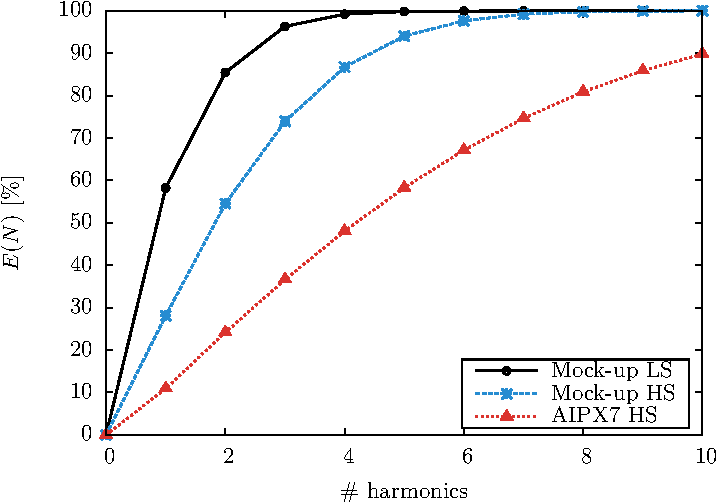
\includegraphics[width=.46\textwidth]{CROR_SPECTRUM_SPAN30.pdf}}\quad
  \subfigure[$50\%$ span]{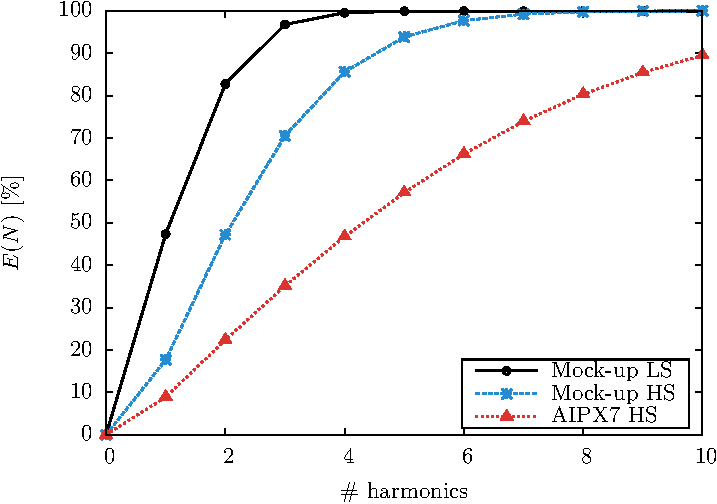
\includegraphics[width=.46\textwidth]{CROR_SPECTRUM_SPAN50.pdf}}\quad
  \subfigure[$70\%$ span]{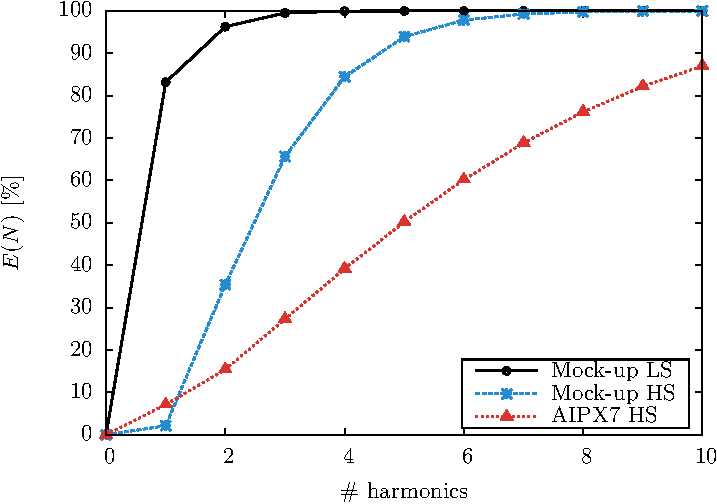
\includegraphics[width=.46\textwidth]{CROR_SPECTRUM_SPAN70.pdf}}\quad
  \subfigure[$90\%$ span]{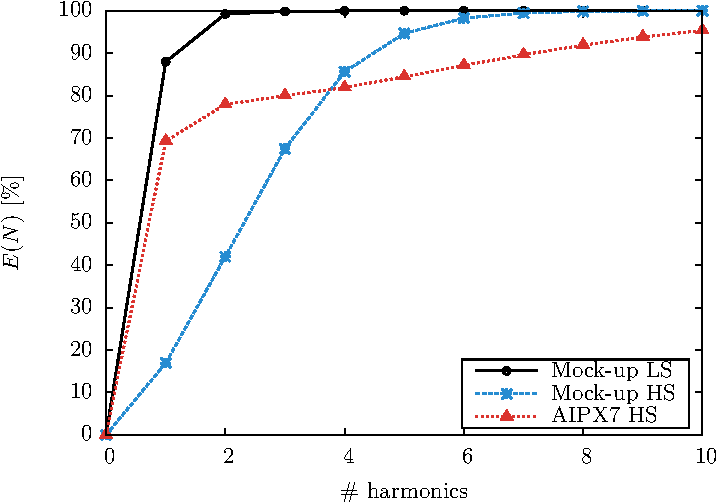
\includegraphics[width=.46\textwidth]{CROR_SPECTRUM_SPAN90.pdf}}\quad
  \caption{Energy accumulation by harmonics at four span positions.}
  \label{fig:crorroxvcurves}
\end{figure}

To have a global insight of the energy contained in the
tangential distortion for all relative span,
the energy accumulation is plotted using a colormap
in Fig.~\ref{fig:crorroxvmapenergy}. This is just
a way to display Fig.~\ref{fig:crorroxvcurves} for all
relative span in one diagram.
Three contour lines are added to ease the
interpretation: $90\%$, $95\%$
and $99\%$, corresponding to a truncation
error of respectively $30\%$, $20\%$ and $10\%$.
\begin{figure}[htbp]
  \centering
  \subfigure[Mock-Up -- Low Speed]{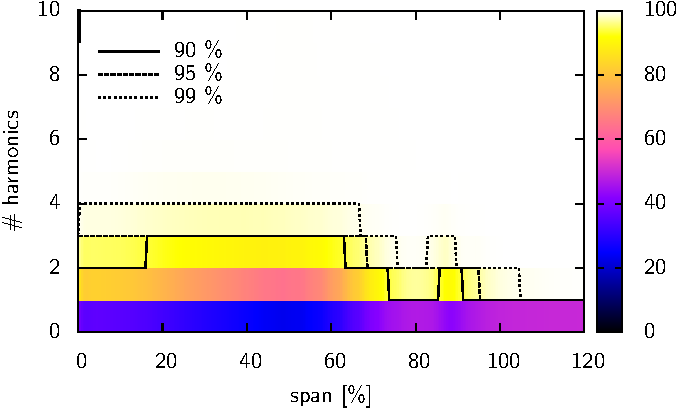
\includegraphics[width=.55\textwidth]{DREAM_LS_RANS_ROE2_SPECTRUM_PPT.pdf}}
  \subfigure[Mock-Up -- High Speed]{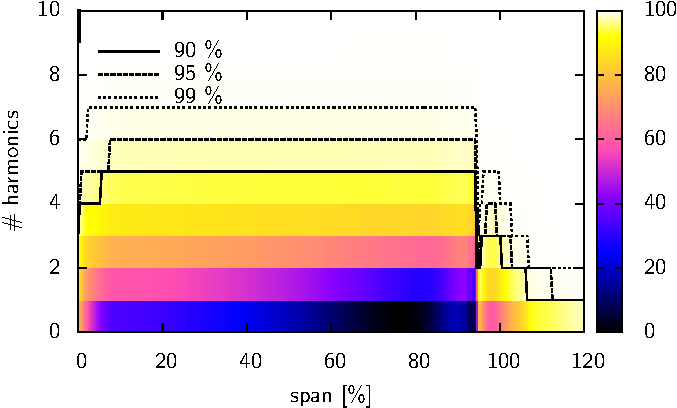
\includegraphics[width=.55\textwidth]{DREAM_HS_RANS_ROE2_SPECTRUM_PPT.pdf}}
  \subfigure[AIPX7 -- High Speed]{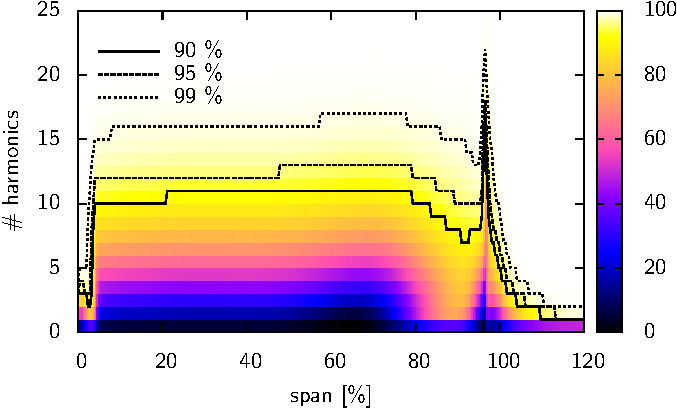
\includegraphics[width=.55\textwidth]{AIPX7_RANS_SPECTRUM_PPT.pdf}}
  \caption{Energy accumulation by harmonics for all spans.}
  \label{fig:crorroxvmapenergy}
\end{figure}
The results are in good agreement with the criterion
based on the wake thickness. In fact, for a relative
span between $10\%$ and $90\%$, the number of harmonics
needed to have $99\%$ of the energy is $4$, $7$ and $16$
for respectively the \mockup LS, the \mockup HS and the
\aipx configurations. This is close to the $2$, $7$ and
$17$ number of harmonics found using a curve fitting
algorithm and the theoretical error derived in 
Sec.~\ref{sec:analytical_considerations}.

This prediction tool is more accurate as it handles
both wake tangential distortion and also any other
type of distortion. Thus, this tool can be used to predict
the number of harmonics needed to capture a certain
level of energy for any relative span.
Moreover, it does take into account for the
viscosity effects, which is not the case of the criteria
proposed in Sec.~\ref{sec:rotating_blocks}.

\subsection{Effect of the numerical scheme}

As one can expect, the numerical scheme used to
compute the configuration has a direct impact on the tangential
distortion seen at the interface. The wake that is 
generated behind the blades of the upstream row is
convected toward the rotor-rotor interface. Depending on
the dissipation and dispersion properties of the numerical
scheme, the wake will be seen different downstream of the
first rotor. Fig.~\ref{fig:crorroxvmap_scheme} shows the azimuthal 
distortions observed depending on the numerical scheme.
Three different schemes are used: a first order, a second
and a theoretical third order Roe scheme. The shape of the
tangential distortion follows the same trend  for the three
schemes but is different locally.
The width of the wake seems almost doubled between the first order
Roe scheme and the third order Roe scheme. This holds true for the tip
vortex foot-print.
\begin{figure}[htbp]
  \centering
  \subfigure[first order Roe scheme]{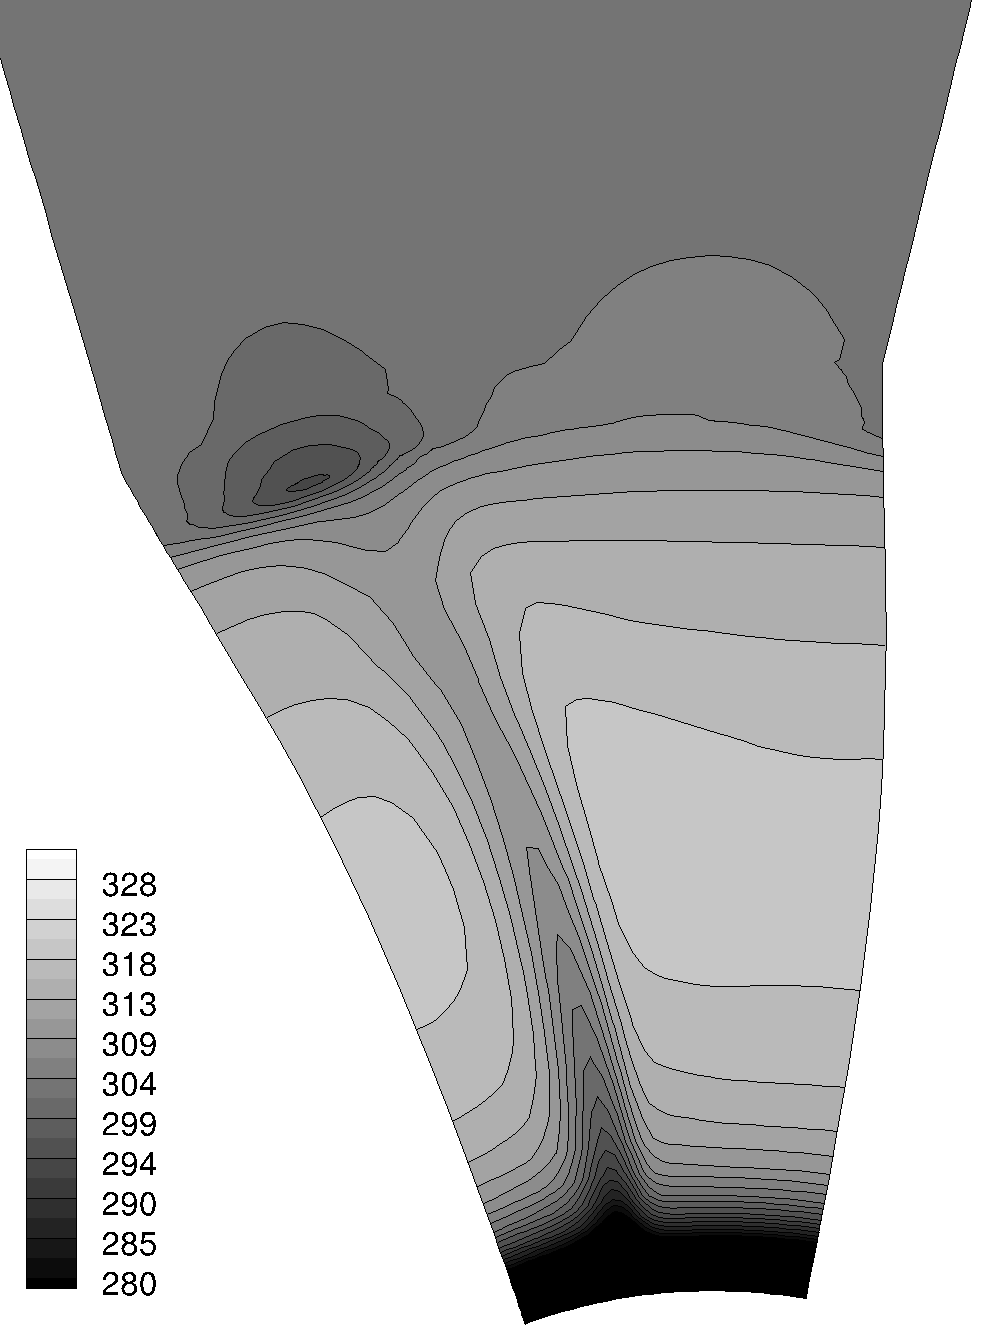
\includegraphics[width=.32\textwidth]{dream_hs_roe1.png}}
  \subfigure[second order Roe scheme]{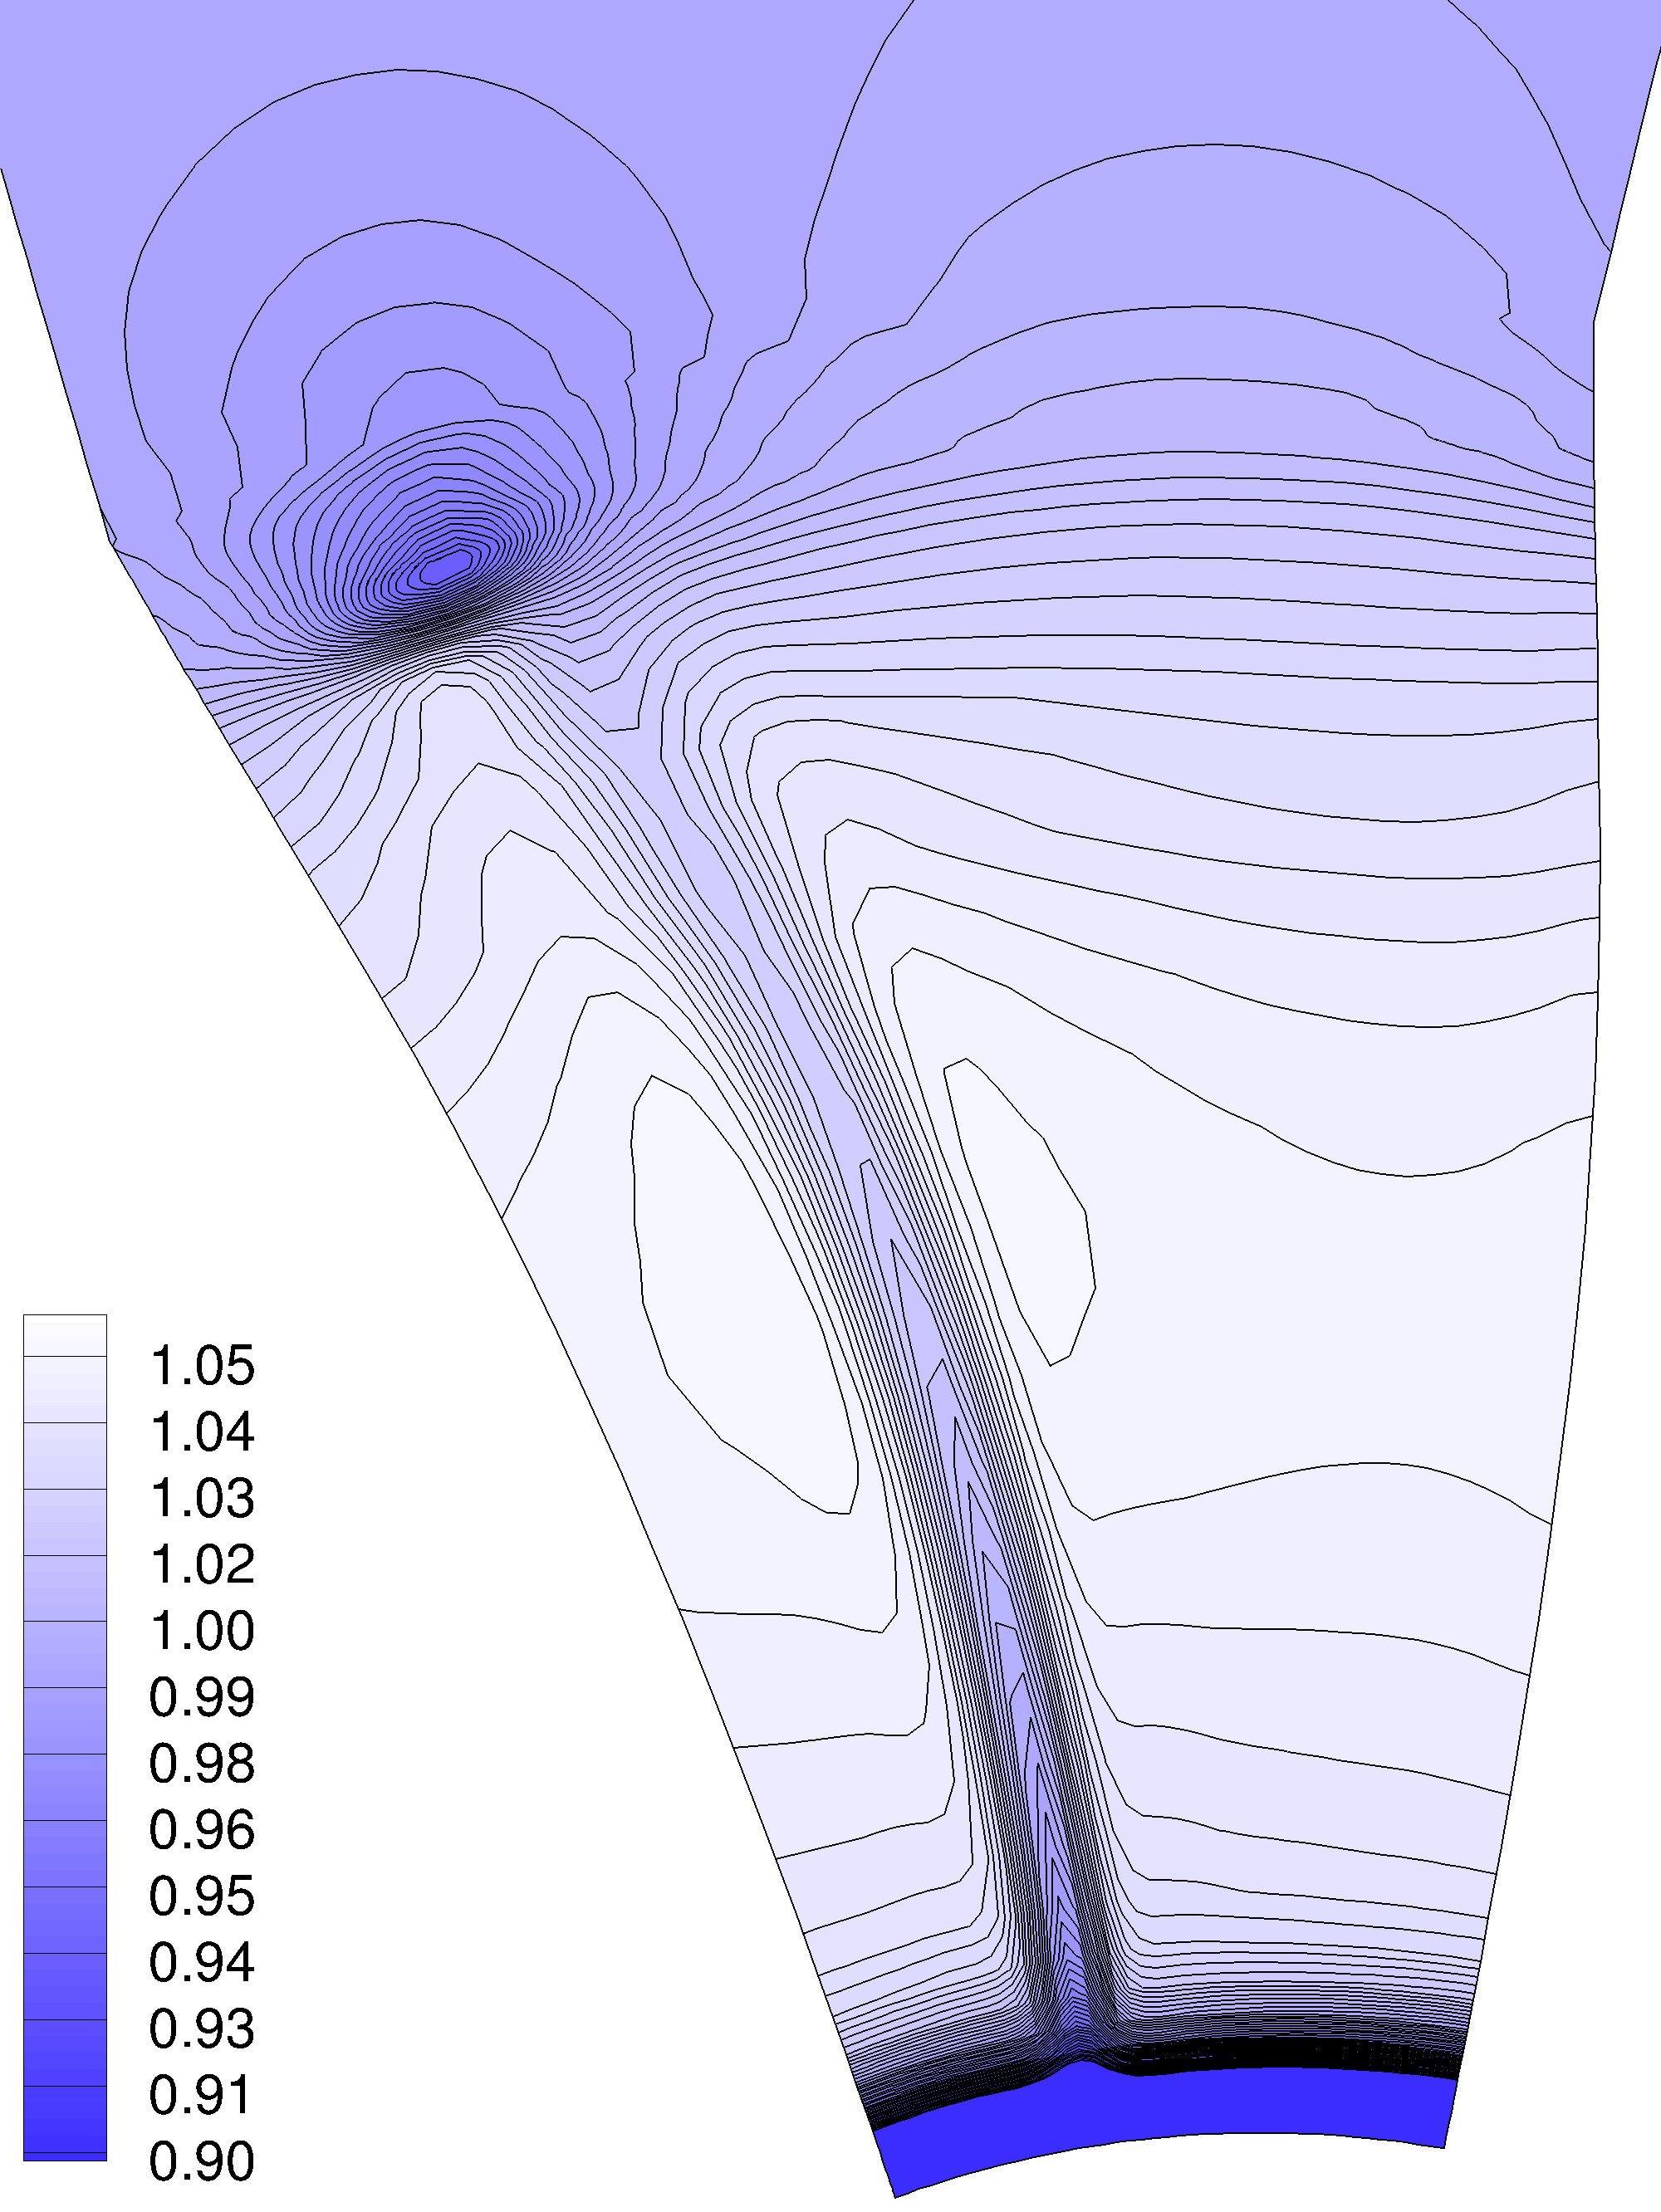
\includegraphics[width=.32\textwidth]{dream_hs_roe2.png}}
  \subfigure[third order Roe scheme]{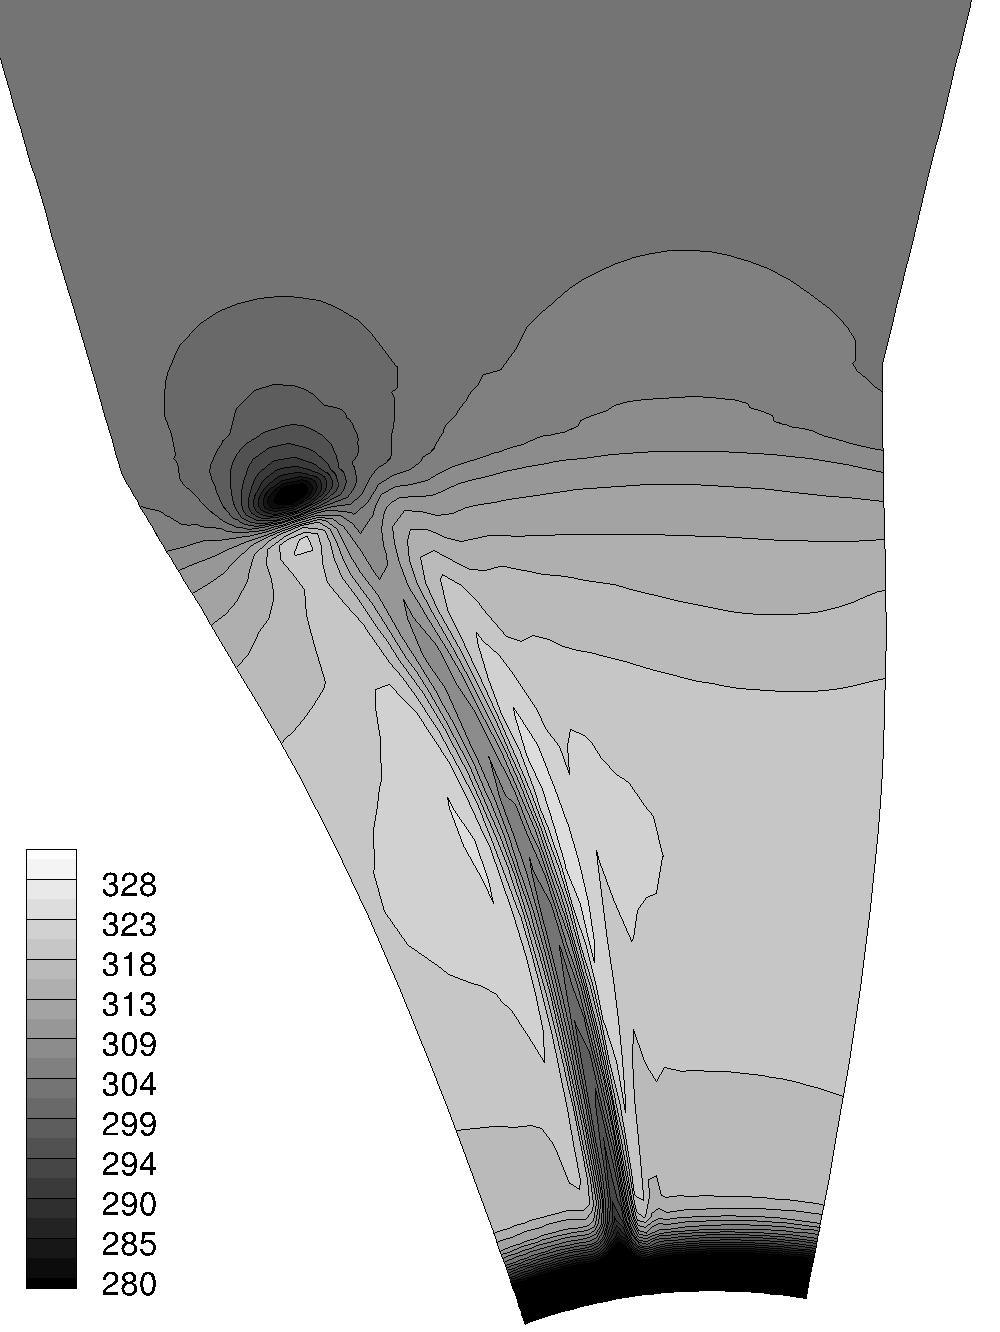
\includegraphics[width=.32\textwidth]{dream_hs_roe3.png}}
  \caption{Non-dimensional axial momentum $(\rho U)/(\rho U)_\infty$ 
  upstream the rotor/rotor interface.}
  \label{fig:crorroxvmap_scheme}
\end{figure}

As the tangential distortion is seen different, the prediction tool
will lead to different conclusions. Fig.~\ref{fig:crorroxvmapenergy_scheme}
shows the application of the prediction tool for the three
different numerical schemes. The conclusions are that
$N=5$, $N=7$ and $N=10$ harmonics are needed to recover 
$99\%$ of the energy for respectively the first order, the 
second order and the third order schemes. This is scattered,
almost as the three CROR configurations were in 
Fig.~\ref{fig:crorroxvmapenergy}. 
\begin{figure}[htbp]
  \centering
  \subfigure[first order Roe scheme]{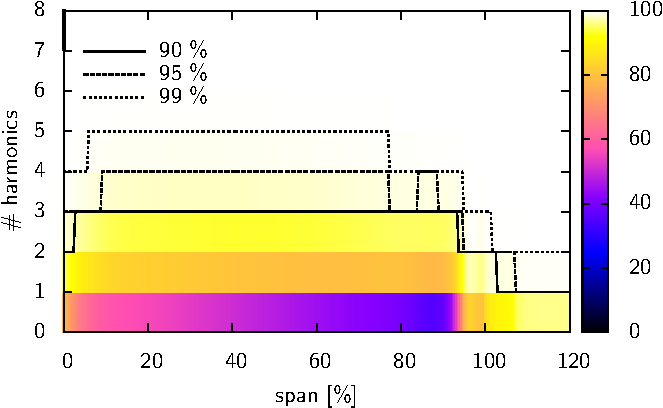
\includegraphics[width=.55\textwidth]{DREAM_HS_RANS_ROE1_SPECTRUM_PPT.pdf}}
  \subfigure[second order Roe scheme]{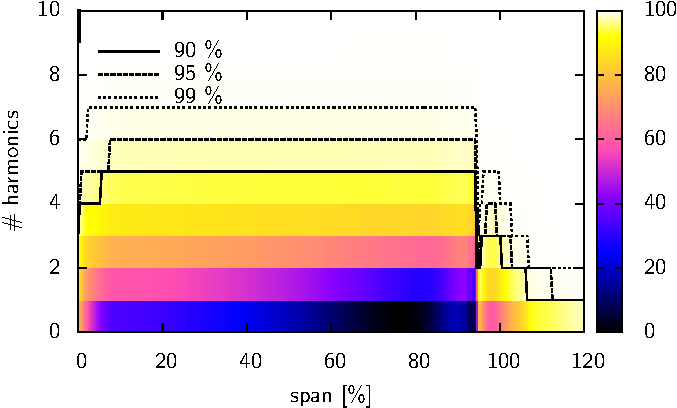
\includegraphics[width=.55\textwidth]{DREAM_HS_RANS_ROE2_SPECTRUM_PPT.pdf}}
  \subfigure[third order Roe scheme]{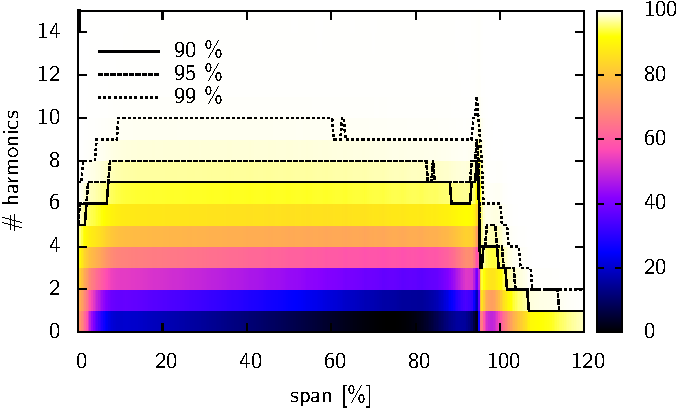
\includegraphics[width=.55\textwidth]{DREAM_HS_RANS_ROE3_SPECTRUM_PPT.pdf}}
  \caption{Effect of the numerical scheme on the energy 
  accumulation at the interface of the \mockup HS configuration.}
  \label{fig:crorroxvmapenergy_scheme}
\end{figure}

Actually, all the numerical or physical parameters
that may lead to a thickening or narrowing of the
wake will be taken into account by the prediction tool.

